% ------------------------------------------------------------------------------
% Este fichero es parte de la plantilla LaTeX para la realización de Proyectos
% Final de Grado, protegido bajo los términos de la licencia GFDL.
% Para más información, la licencia completa viene incluida en el
% fichero fdl-1.3.tex

% Copyright (C) 2012 SPI-FM. Universidad de Cádiz
% ------------------------------------------------------------------------------

\section{Introducción}
En esta sección describiremos lo más sustancial para entender el funcionamiento del sistema. Cualquier duda que tenga el usuario de la aplicación sobre el funcionamiento de la misma podrá resolverla haciendo uso de este manual o poniéndose en contacto con el desarrollador de la aplicación.

\section{Utilización}

\subsection {Pantalla de logueo}
Para poder hacer uso de todas las funcionalidades del sistema, el usuario de la aplicación debe loguearse en ella mediante la pantalla de login:

\begin{figure}[!htb]
  \centering
    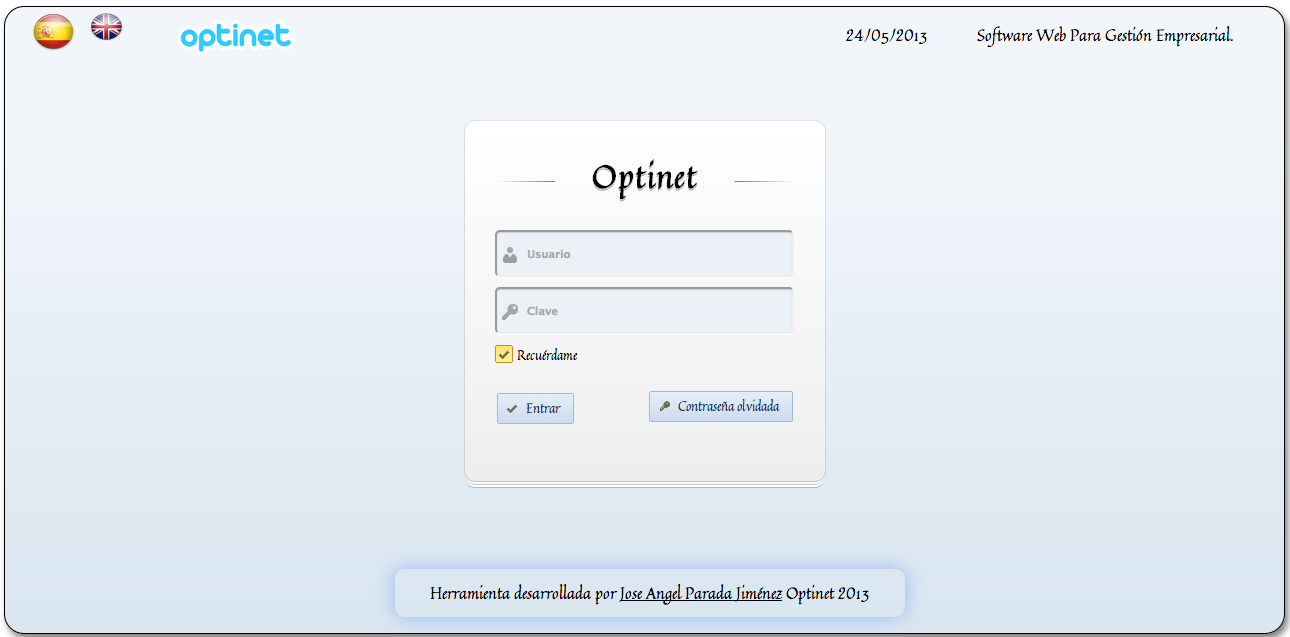
\includegraphics[scale=0.35]{caplogin.png}
  \caption{Pantalla logueo}
  \label{a}
\end{figure}

En esta pantalla ya se puede intuir el aspecto que tendrá la aplicación en las demás pantallas. Cualquier error en el formulario de login aparecerá debajo de los botones. Al usuario se le da la posibilidad de recordar la contraseña, si esta opción está marcada se recordará su contraseña durante 30 minutos. El usuario puede mandar un email al desarrollador de la aplicación pulsando en la parte inferior en el nombre. En la parte superior, que estará visible en las demás pantallas, se puede ver el usuario conectado, el rol que posee y la fecha actual. El usuario puede cambiar de idioma en cualquier pantalla de la aplicación, incluyendo ésta de logueo. Dependiendo del rol del usuario que se conecte el sistema mostrará solo las acciones que ese usuario puede realizar:
\begin{itemize}
\item Administrador: Se mostrará en el menú superior un desplegable con nombre Admin.
\item Médico: Se mostrará la opción de crear informes en el menú informes
\end{itemize}

\subsection {Pantalla de contraseña olvidada}

\begin{figure}[!htb]
  \centering
    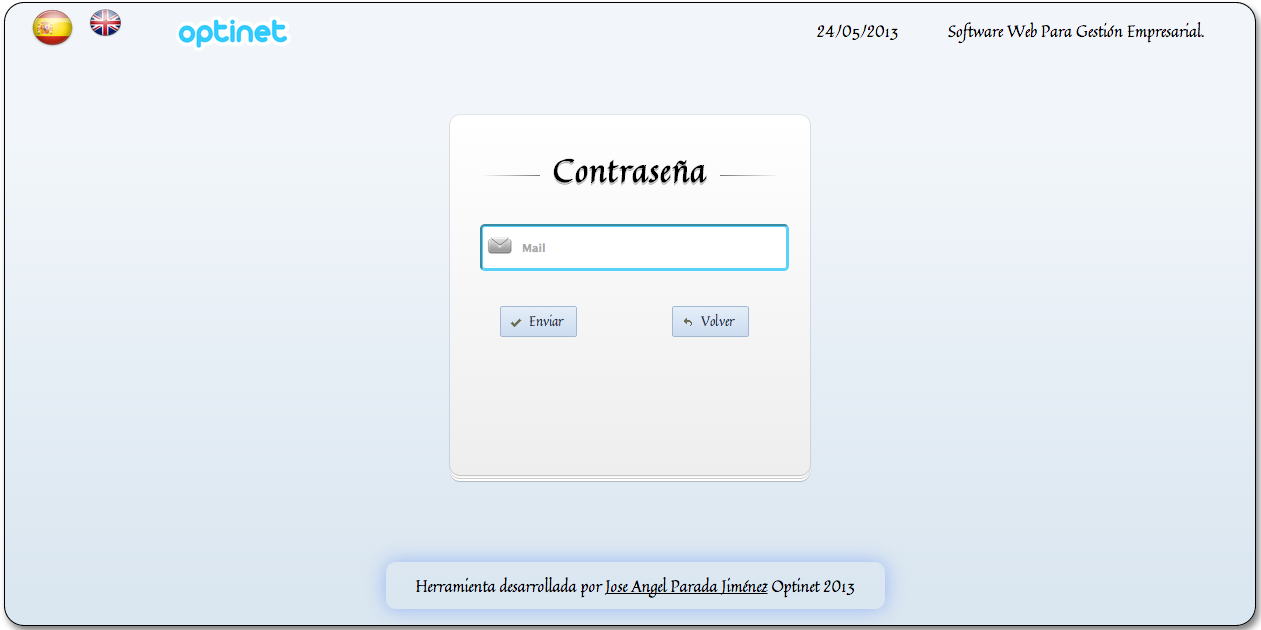
\includegraphics[scale=0.35]{capolvidada.png}
  \caption{Pantalla contraseña olvidada}
  \label{a}
\end{figure}

En esta pantalla cualquier usuario de la aplicación puede recuperar su contraseña olvidada indicando su email. El sistema le mandará un email con un enlace de reestablecimiento de la contraseña al email el cual solo valdrá para un solo uso. Si se pulsase en ese enlace se generará una nueva contraseña para el usuario y se le enviará la nueva contraseña a su email. Debajo de los botones se podrá ver si se ha mandado el email o por el contrario ha ocurrido algún error.

\newpage
\subsection {Pantalla principal}

\begin{figure}[!htb]
  \centering
    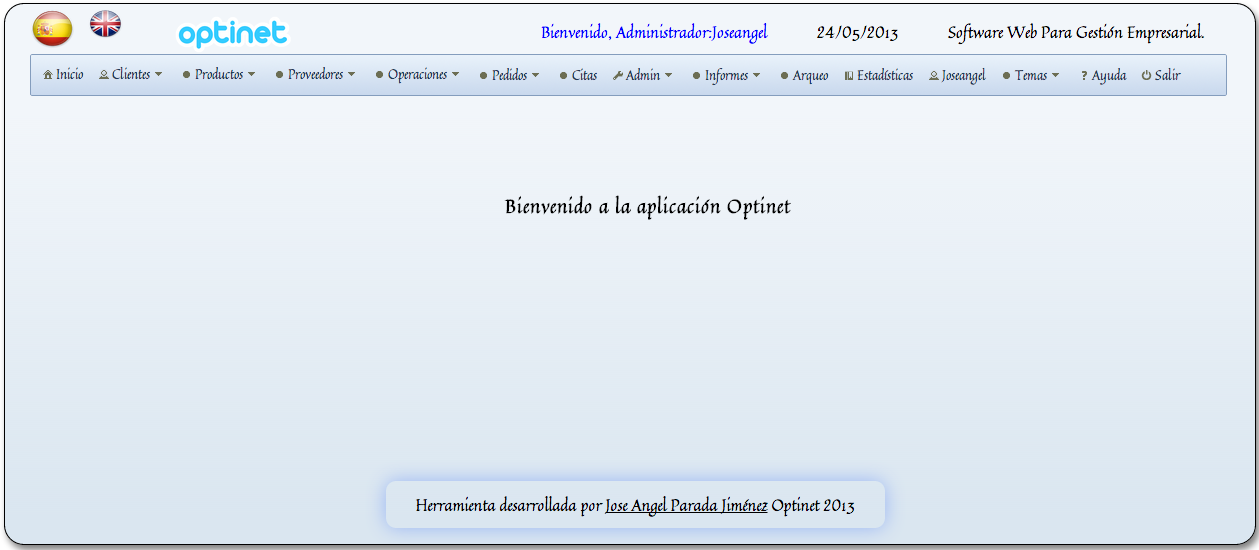
\includegraphics[scale=0.35]{capprincipal.png}
  \caption{Pantalla principal}
  \label{a}
\end{figure}

Esta es la pantalla que el usuario de la aplicación ve al loguearse en el sistema correctamente. Aquí el usuario ya puede usar toda la funcionalidad del sistema incluyendo cambiar de idioma o cambiar el tema visual.

\subsection {Pantalla registro cliente}

\begin{figure}[!htb]
  \centering
    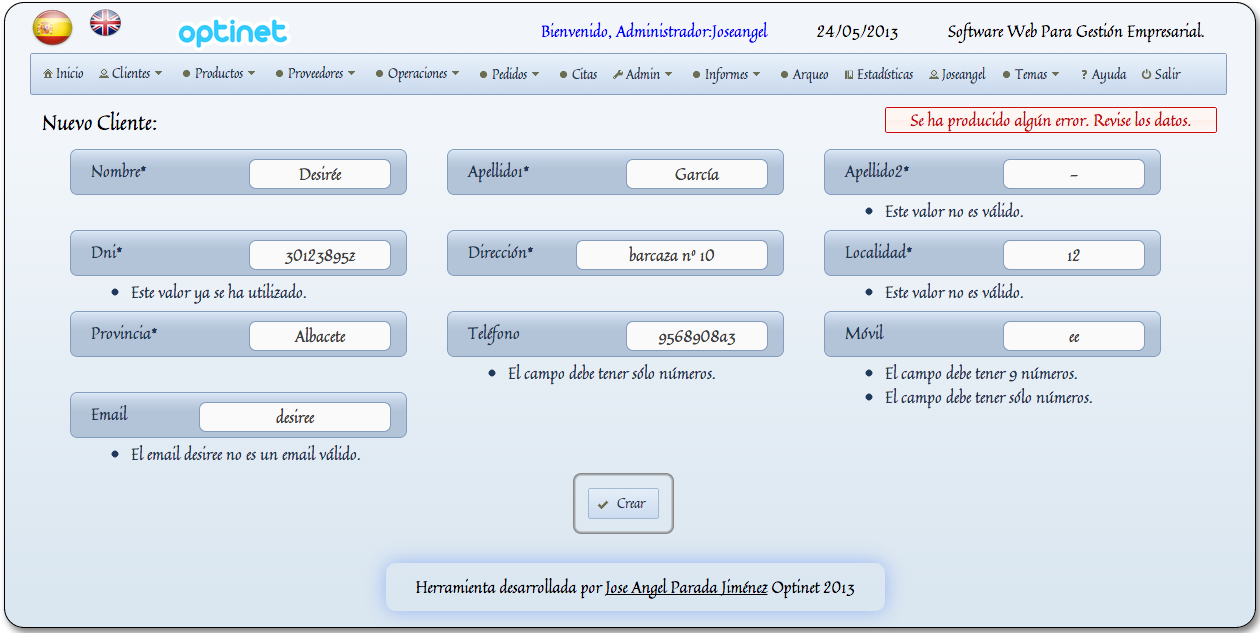
\includegraphics[scale=0.35]{capregistrocliente.png}
  \caption{Pantalla registro cliente}
  \label{a}
\end{figure}

En esta pantalla el usuario de la aplicación puede registrar a un nuevo cliente en el sistema. Si se produce algún tipo de error en la introducción de datos se mostrará un mensaje de error en la parte superior derecha de la pantalla y se verán reflejados los errores debajo de cada campo de inserción.

\subsection {Pantalla listar clientes}

\begin{figure}[!htb]
  \centering
    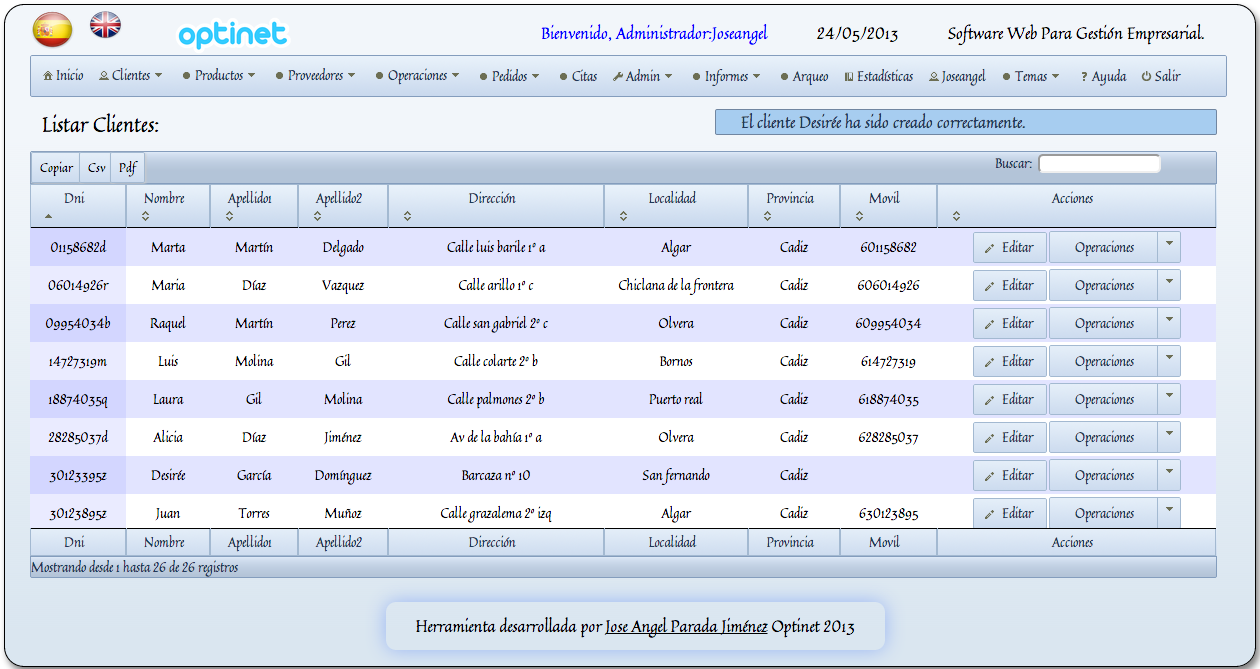
\includegraphics[scale=0.35]{caplistarclientes.png}
  \caption{Pantalla listar clientes}
  \label{a}
\end{figure}

En esta pantalla el usuario de la aplicación puede consultar los clientes almacenados en el sistema. La tabla ofrece la opción al usuario de ordenar cualquier columna o buscar en el campo situado en la parte superior derecha de la tabla. Además, ofrece la posibilidad de copiar al portapapeles, copiar en formato CSV, o un documento PDF de los datos mostrados en la tabla. El usuario puede realizar alguna opción con el cliente pulsando en el desplegable operaciones. Cuando se crea, modifica, o elimina a un cliente del sistema se redirigirá al usuario de la aplicación a esta página donde podrá ver el mensaje de éxito de la operación en la parte superior derecha.

\newpage
\subsection {Pantalla modificar cliente}

\begin{figure}[!htb]
  \centering
    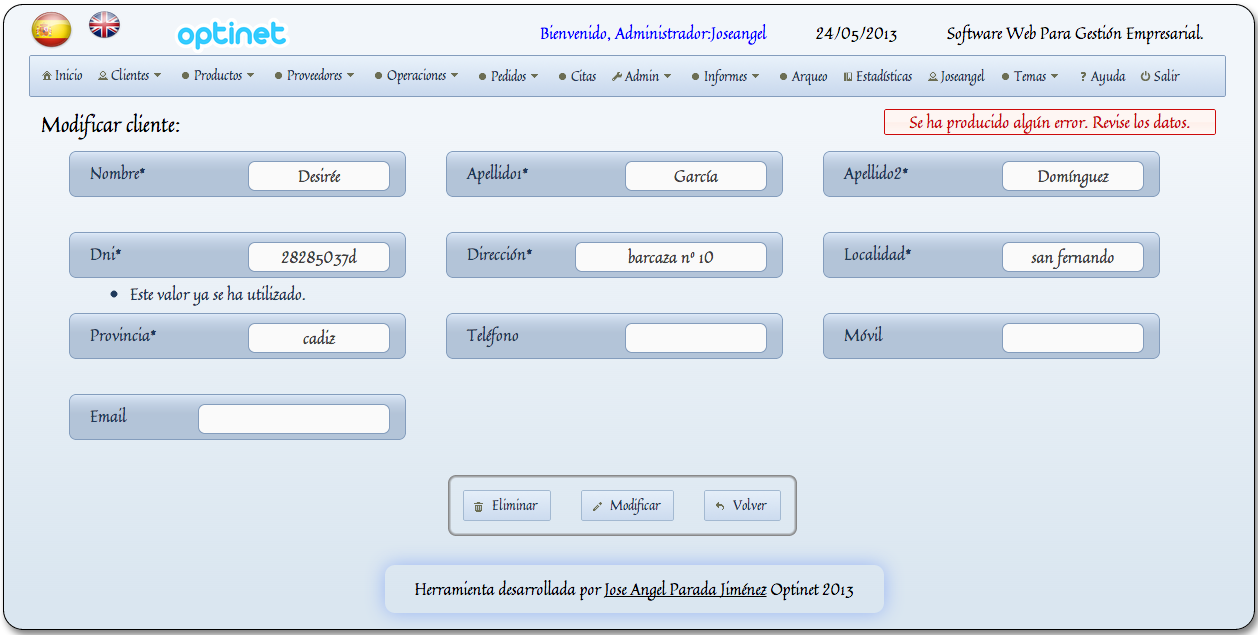
\includegraphics[scale=0.35]{capmodificarcliente.png}
  \caption{Pantalla modificar cliente}
  \label{a}
\end{figure}

En esta pantalla el usuario de la aplicación puede modificar a un cliente en el sistema. Si se produce algún tipo de error en la introducción de datos se mostrará un mensaje de error en la parte superior derecha de la pantalla y se verán reflejados los errores debajo de cada campo de inserción. En esta pantalla además ofrece la posibilidad de eliminar a un cliente del sistema, teniendo en cuenta que solo se podrán eliminar si no tiene operaciones asociadas, en caso contrario se mostrará el botón desactivado y aparecerá un mensaje indicándolo al poner el cursor sobre el botón desactivado.

\newpage
\subsection {Pantalla mover productos}

\begin{figure}[!htb]
  \centering
    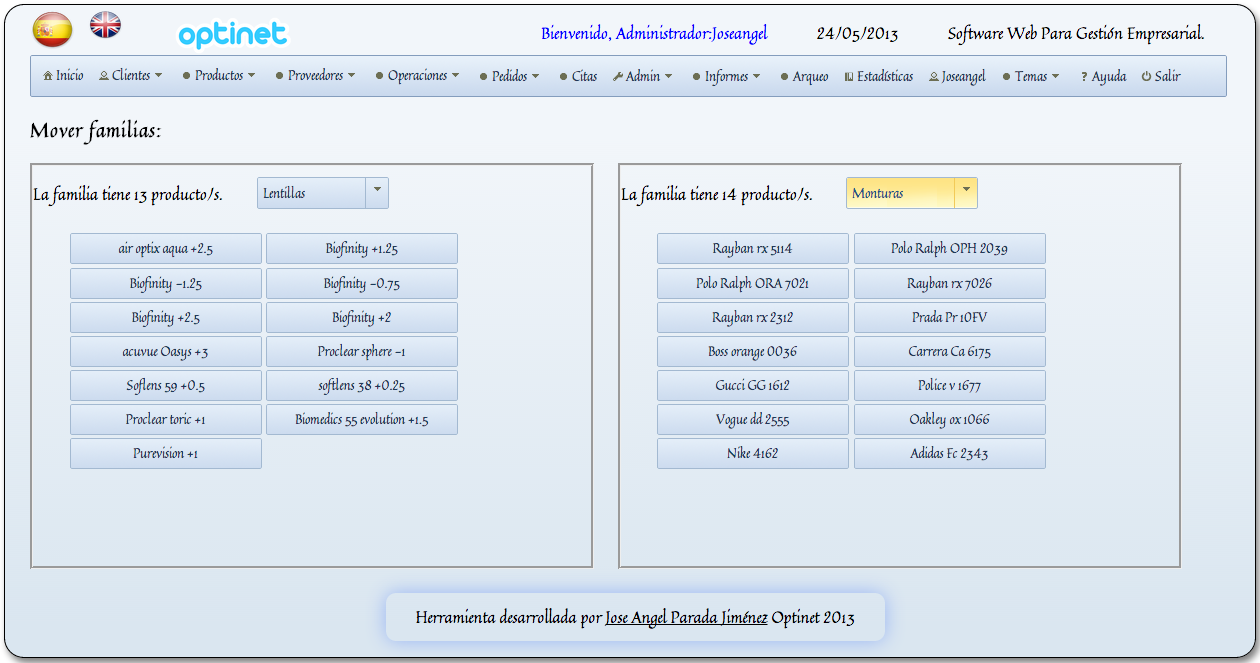
\includegraphics[scale=0.35]{capmoverproductos.png}
  \caption{Pantalla mover productos}
  \label{a}
\end{figure}

En esta pantalla el usuario de la aplicación puede mover los productos del sistema entre familias. El usuario podrá arrastrar los productos a la familia que desee o dejarlos sin familia ya que en el desplegable también aparece la opción de productos sin familia.

\subsection {Pantalla registrar producto}

\begin{figure}[!htb]
  \centering
    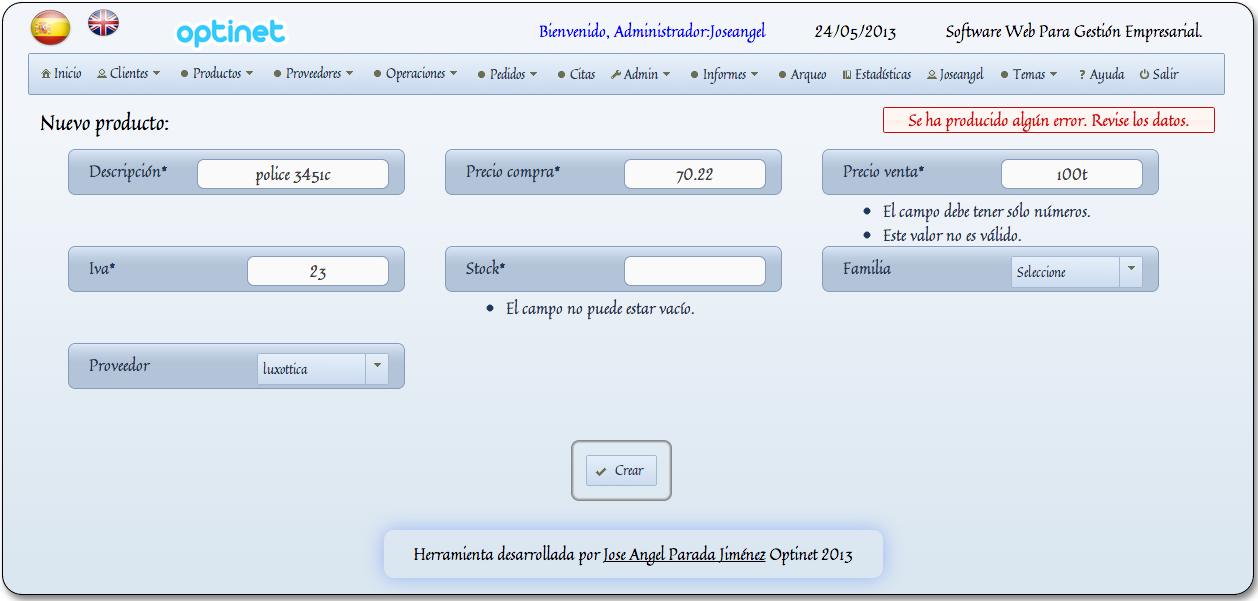
\includegraphics[scale=0.35]{capregistroproducto.png}
  \caption{Pantalla registrar productos}
  \label{a}
\end{figure}

En esta pantalla el usuario de la aplicación puede registrar a un producto en el sistema. Si se produce algún tipo de error en la introducción de datos se mostrará un mensaje de error en la parte superior derecha de la pantalla y se verán reflejados los errores debajo de cada campo de inserción. El usuario puede insertar un nuevo producto sin indicar la familia a la que pertenece o el proveedor que suministra ese producto.


\subsection {Pantalla modificar producto}

\begin{figure}[!htb]
  \centering
    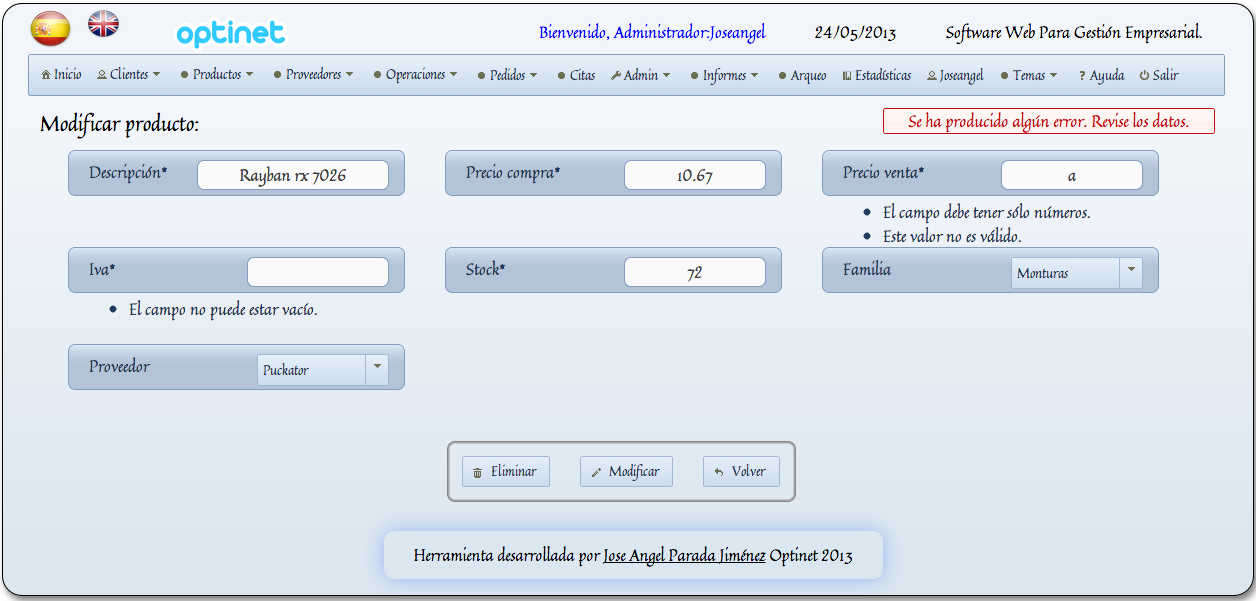
\includegraphics[scale=0.35]{capmodificarproducto.png}
  \caption{Pantalla modificar producto}
  \label{a}
\end{figure}

En esta pantalla el usuario de la aplicación puede modificar a un producto en el sistema. Si se produce algún tipo de error en la introducción de datos se mostrará un mensaje de error en la parte superior derecha de la pantalla y se verán reflejados los errores debajo de cada campo de inserción. En esta pantalla además ofrece la posibilidad de eliminar a un producto del sistema, teniendo en cuenta que solo se podrán eliminar si no tiene operaciones asociadas, en caso contrario se mostrará el botón desactivado y aparecerá un mensaje indicándolo al poner el cursor sobre el botón desactivado.
\newpage
\subsection {Pantalla listar productos}

\begin{figure}[!htb]
  \centering
    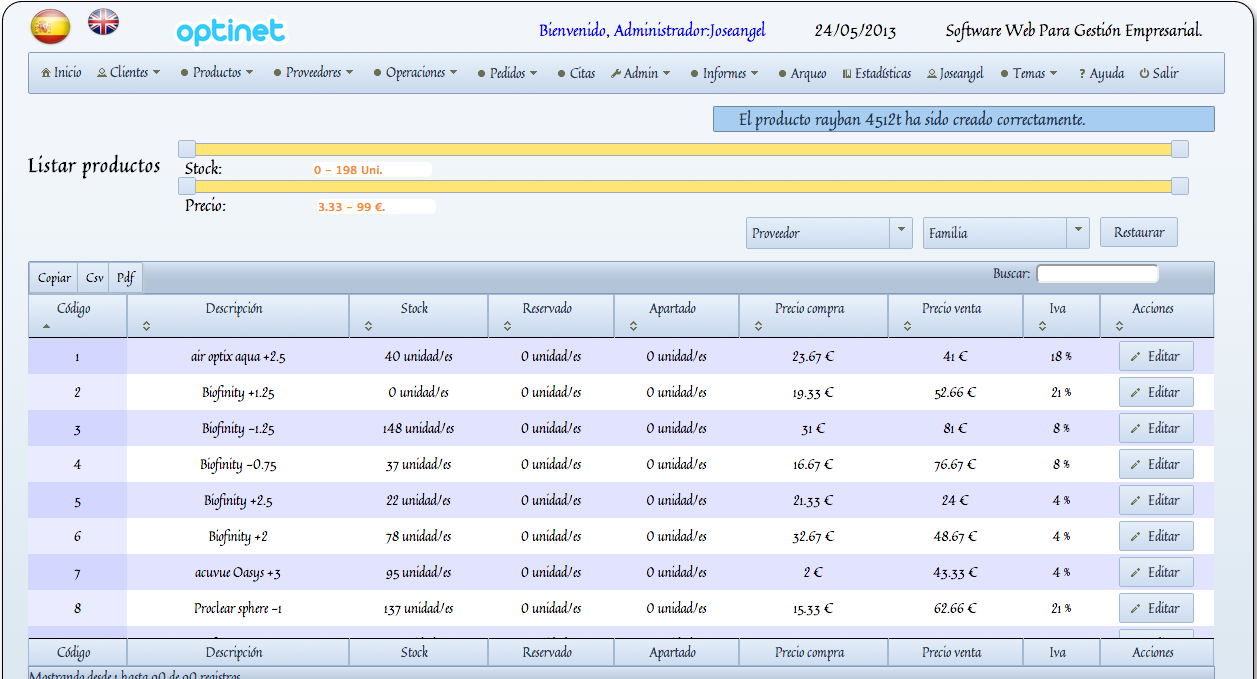
\includegraphics[scale=0.35]{caplistarproductos.png}
  \caption{Pantalla listar productos}
  \label{a}
\end{figure}

En esta pantalla el usuario de la aplicación puede consultar los productos almacenados en el sistema. La tabla ofrece la opción al usuario de ordenar cualquier columna o buscar en el campo situado en la parte superior derecha de la tabla. Además ofrece la posibilidad de copiar al portapapeles, copiar en formato csv, o un documento pdf de los datos mostrados en la tabla. En la parte superior el usuario podrá realizar filtrados a la tabla modificando los desplegables o los sliders. Cuando se crea, modifica o elimina a un producto del sistema se redirigirá al usuario de la aplicación a esta página donde podrá ver el mensaje de éxito de la operación en la parte superior derecha.

\newpage
\subsection {Pantalla listar familias}

\begin{figure}[!htb]
  \centering
    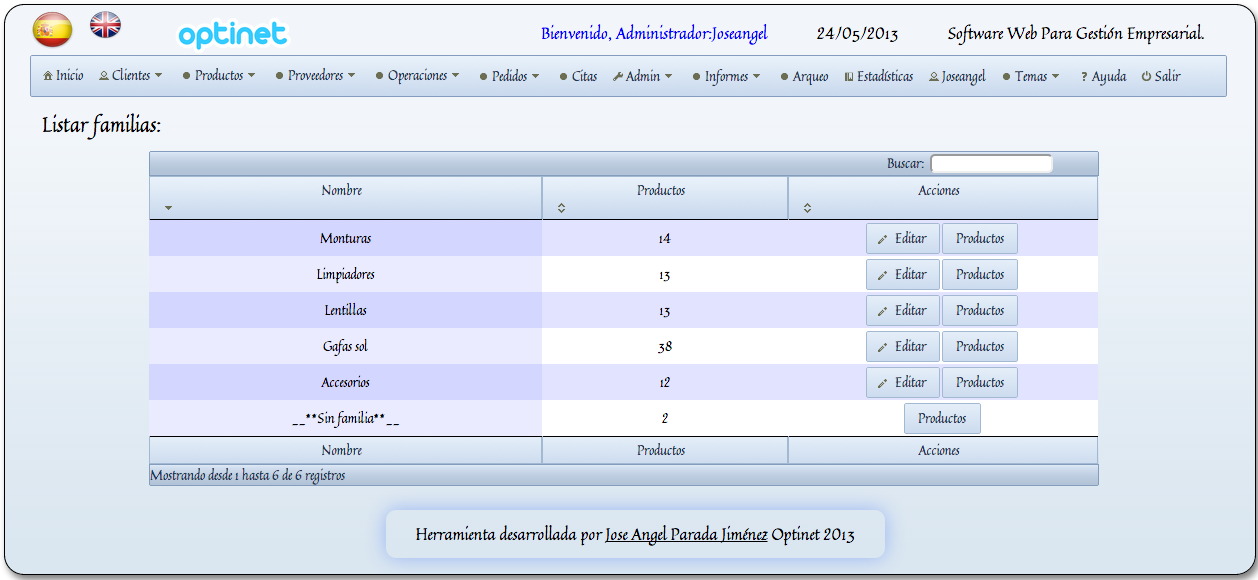
\includegraphics[scale=0.35]{caplistarfamilias.png}
  \caption{Pantalla listar familias}
  \label{a}
\end{figure}

En esta pantalla el usuario de la aplicación puede consultar las familias almacenadas en el sistema. Se ofrece la posibilidad al usuario de poder consultar los productos de una determinada familia pulsando en el botón Productos. Esta opción está también disponible en la pantalla listar proveedores para consultar los productos que suministra un determinado proveedor.

\newpage
\subsection {Pantalla nueva venta}

\begin{figure}[!htb]
  \centering
    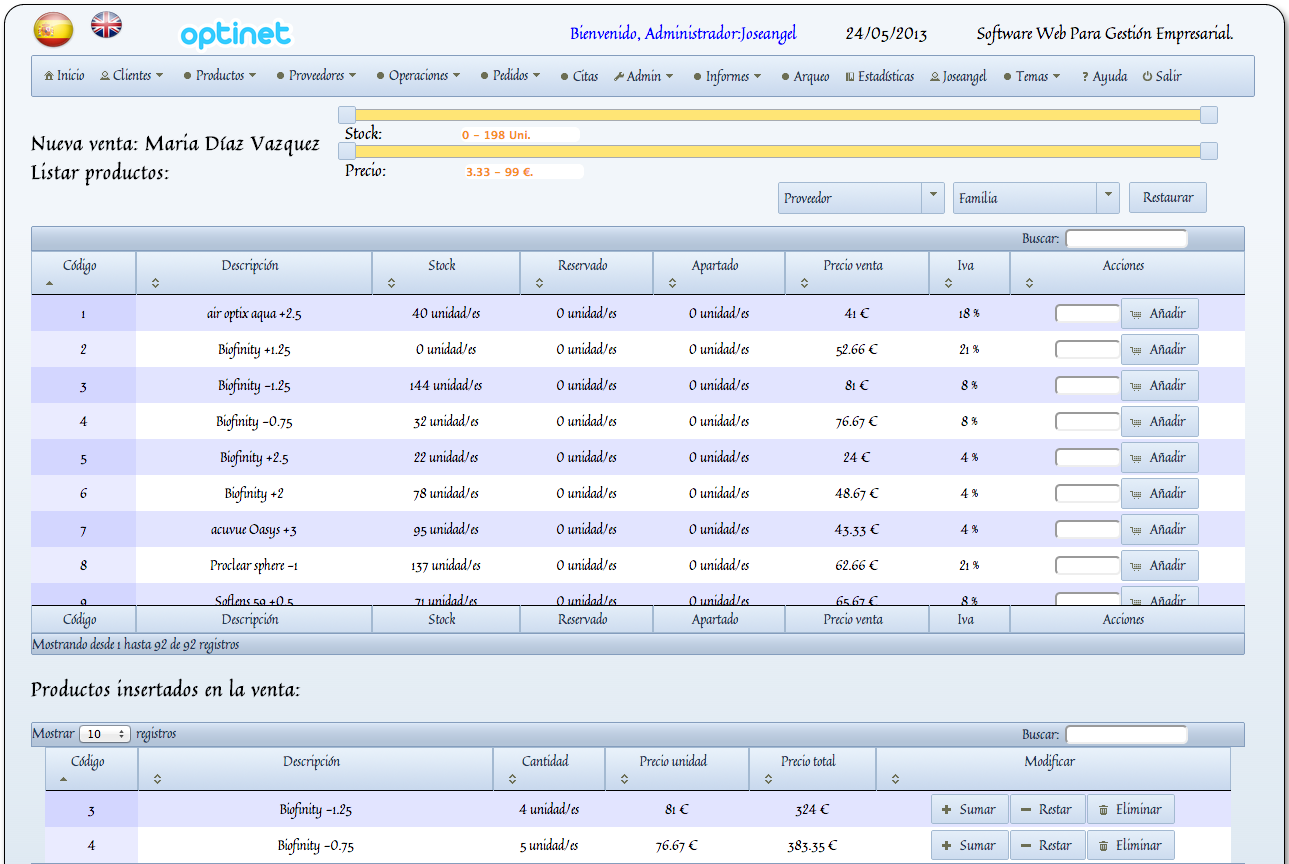
\includegraphics[scale=0.35]{capnuevaventa.png}
  \caption{Pantalla nueva venta}
  \label{a}
\end{figure}

\begin{figure}[!htb]
  \centering
    
\includegraphics[scale=0.35]{capnuevaventa1.png}
  \caption{Pantalla nueva venta1}
  \label{a}
\end{figure}

\begin{figure}[!htb]
  \centering
    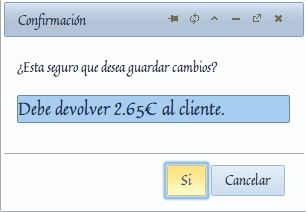
\includegraphics[scale=0.35]{capnuevaventa2.png}
  \caption{Pantalla nueva venta2}
  \label{a}
\end{figure}

En esta pantalla el usuario de la aplicación puede crear una nueva venta en el sistema. Primeramente se mostrará una tabla donde el usuario elegirá al cliente que quiere realizar una venta. En la parte superior el usuario podrá realizar filtrados a la tabla modificando los desplegables o los sliders. A medida que se vayan indicando productos se irán mostrando en la tabla inferior y podremos aumentar, decrementar o eliminar alguno de esos productos desde esa misma tabla. Cualquier dato introducido de manera incorrecta se mostrará un mensaje de error. El usuario puede elegir si mostrar en ese mismo instante el documento de venta o la forma de pago del cliente, efectivo o tarjeta. Si fuese tarjeta el campo de texto entregado desaparecería. Al pulsar el botón guardar se mostrará un mensaje para confirmar la venta, éste mensaje incluirá el importe a devolver al cliente si se escogió pago en efectivo, en caso contrario solo mostrará el mensaje de confirmación. Una vez que se haya efectuado la venta se redigirá al usuario a la lista de ventas.

\subsection {Pantalla listar ventas}

\begin{figure}[!htb]
  \centering
    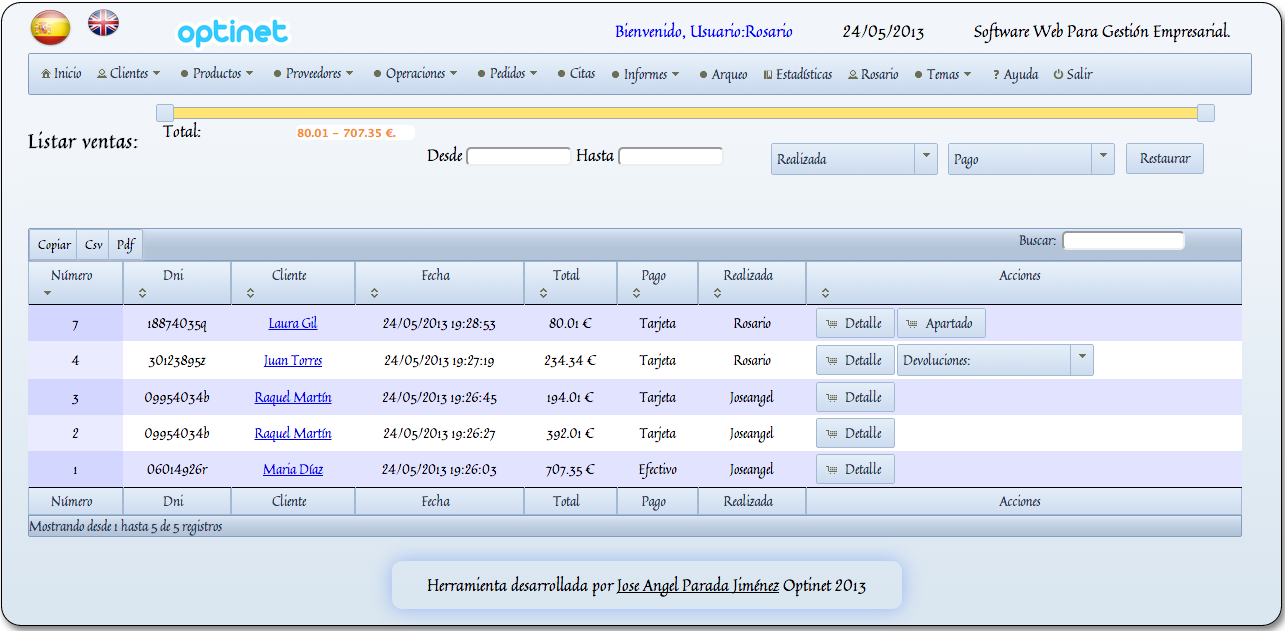
\includegraphics[scale=0.35]{caplistarventas.png}
  \caption{Pantalla listar ventas}
  \label{a}
\end{figure}

En esta pantalla el usuario de la aplicación puede ver las ventas creadas en el sistema. Se da al usuario la posibilidad de hacer filtrados a la tabla con los desplegables y sliders de la parte superior, incluyendo también hacer un filtrado de un rango de fechas. El usuario puede ver el detalle de una determinada venta, mostrándose los productos asociados, el documento de venta y también puede, pulsando sobre el nombre del cliente, ver más datos del cliente. También puede mostrar, si existe, la devolución de una venta pulsando en el desplegable devoluciones.

\newpage
\subsection {Pantalla nueva devolución}

\begin{figure}[!htb]
  \centering
    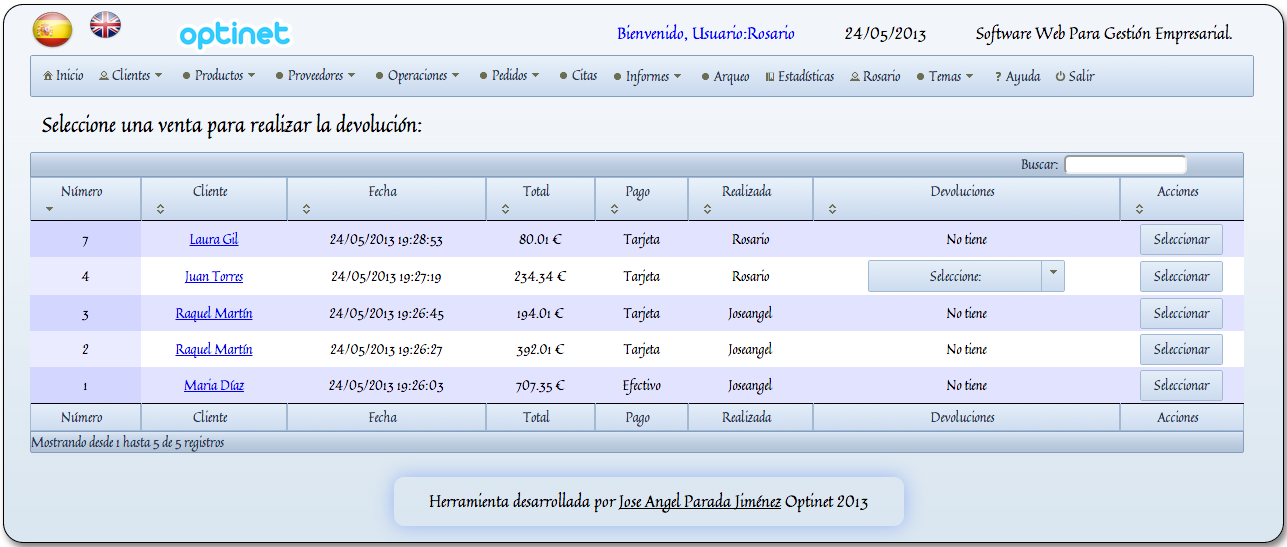
\includegraphics[scale=0.35]{capnuevadevolucion.png}
  \caption{Pantalla nueva devolución}
  \label{a}
\end{figure}

\begin{figure}[!htb]
  \centering
    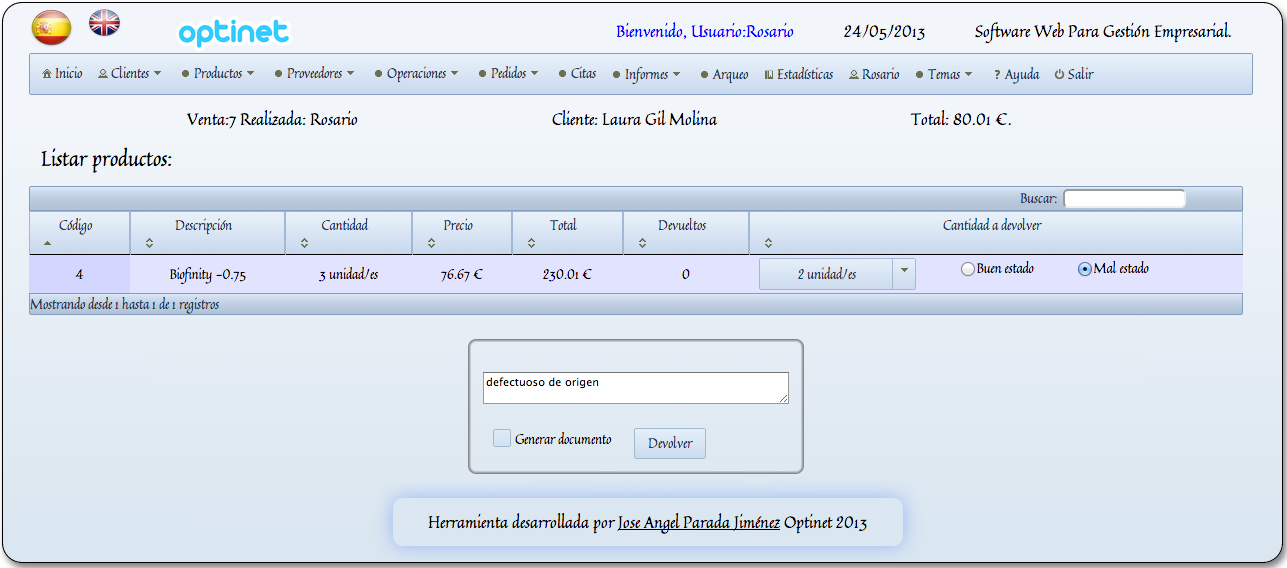
\includegraphics[scale=0.35]{capnuevadevolucion1.png}
  \caption{Pantalla nueva devolución1}
  \label{a}
\end{figure}

En esta pantalla el usuario de la aplicación puede crear una nueva devolución en el sistema. Primeramente se mostrará una tabla donde el usuario elegirá la venta a la que quiere realizar la devolución. El usuario seleccionará las cantidades de los productos de esa venta que quiere devolver y su estado. Si el estado es bueno, se aumentarían los stocks. La forma de devolución al cliente será la misma con la que se hizo la venta. El usuario puede elegir si mostrar en ese mismo instante el documento de devolución. Al pulsar el botón guardar se mostrará un mensaje para confirmar la devolución. Una vez que se haya efectuado la devolución se redigirá al usuario a la lista de devoluciones.

\newpage
\subsection {Pantalla listar reservas}

\begin{figure}[!htb]
  \centering
    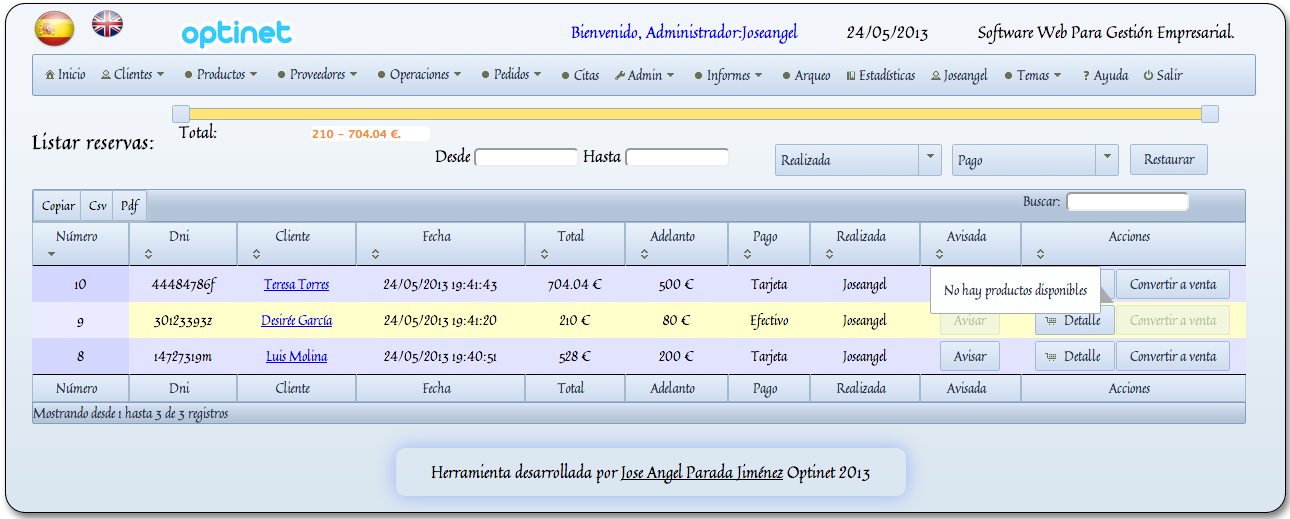
\includegraphics[scale=0.35]{caplistarreservas.png}
  \caption{Pantalla listar reservas}
  \label{a}
\end{figure}

En esta pantalla el usuario de la aplicación puede ver las reservas creadas en el sistema. Se da al usuario la posibilidad de hacer filtrados a la tabla con los desplegables y sliders de la parte superior, incluyendo también hacer un filtrado de un rango de fechas. El usuario puede ver el detalle de una determinada reserva, mostrándose los productos asociados, el documento de reserva y también puede, pulsando sobre el nombre del cliente, ver más datos del cliente. El usuario puede convertir en venta una reserva si los productos están ya disponibles o registrar el aviso al cliente para que venga a recoger la reserva. Si no se pudiese avisar al cliente porque los productos no están disponibles o porque la reserva ya se ha convertido en venta, el botón avisar aparecerá desactivado.

\newpage
\subsection {Pantalla listar operaciones}

\begin{figure}[!htb]
  \centering
    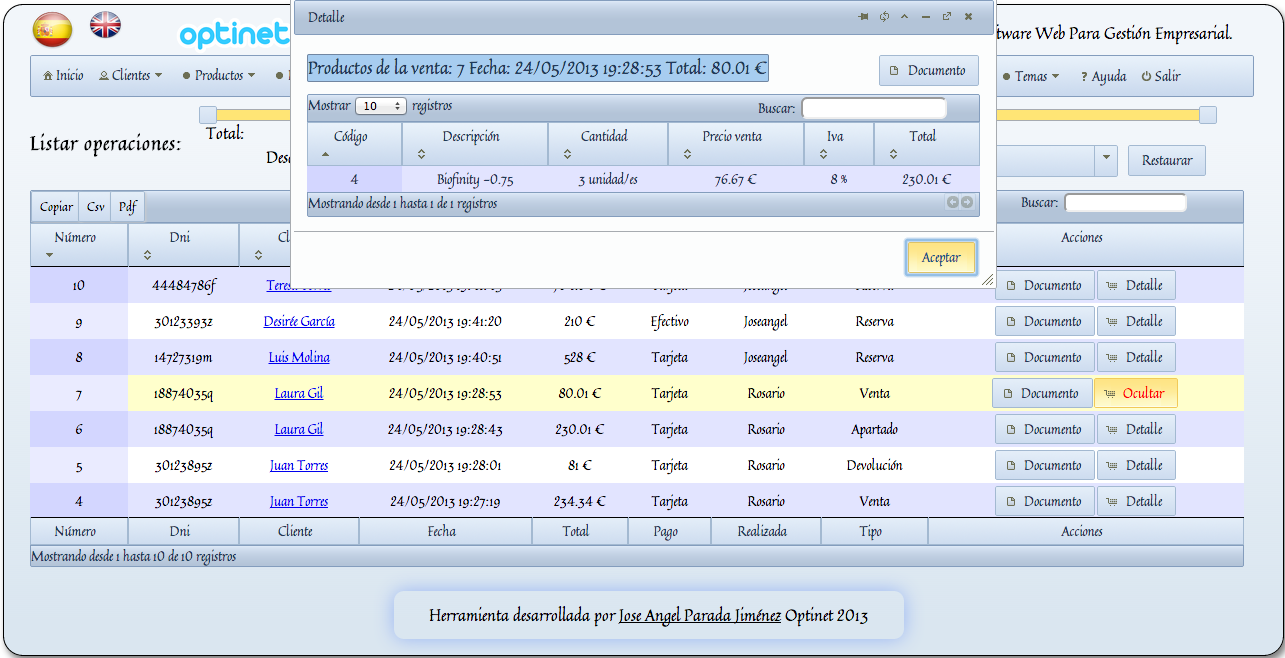
\includegraphics[scale=0.35]{caplistaroperaciones.png}
  \caption{Pantalla listar operaciones}
  \label{a}
\end{figure}

En esta pantalla el usuario de la aplicación puede ver todas las operaciones creadas en el sistema(venta, devolución, reserva, apartado). Se da al usuario, como siempre, la posibilidad para realizar los filtrados que son necesarios para realizar búsquedas y también indicar que en esta pantalla, por ejemplo, se podrían ver las operaciones que ha efectuado un cliente determinado. El usuario podría ver el documento asociado al tipo de operación pulsando en documento, o podría ver los productos asociados a una operación determinada pulsando en el botón detalle.

\newpage
\subsection {Pantalla nuevo pedido}

\begin{figure}[!htb]
  \centering
    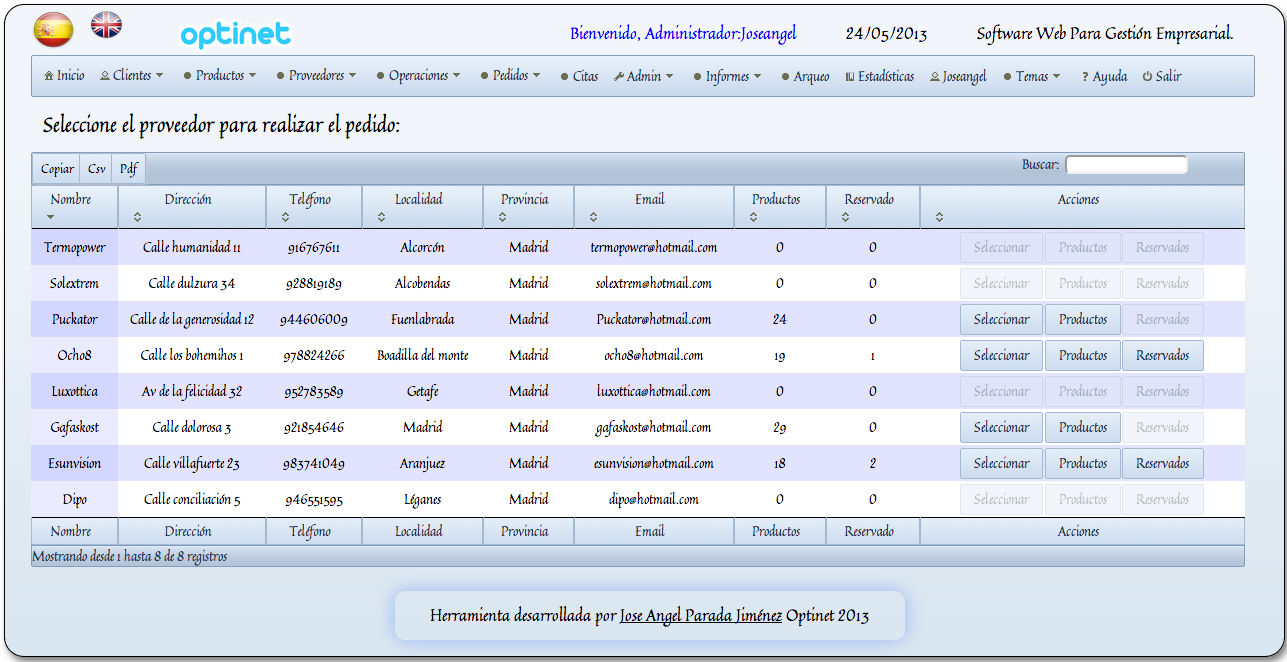
\includegraphics[scale=0.35]{capnuevopedido.png}
  \caption{Pantalla nuevo pedido}
  \label{a}
\end{figure}

En esta pantalla el usuario de la aplicación puede crear un nuevo pedido a un determinado proveedor. Primero se le mostrará al usuario una pantalla donde podrá ver los proveedores que tienen algún producto reservado, consultar los productos que suministra cada proveedor o ver en que reserva están los productos reservados. El usuario deberá seleccionar el proveedor al que quiere hacerle un pedido. 

\newpage
\begin{figure}[!htb]
  \centering
    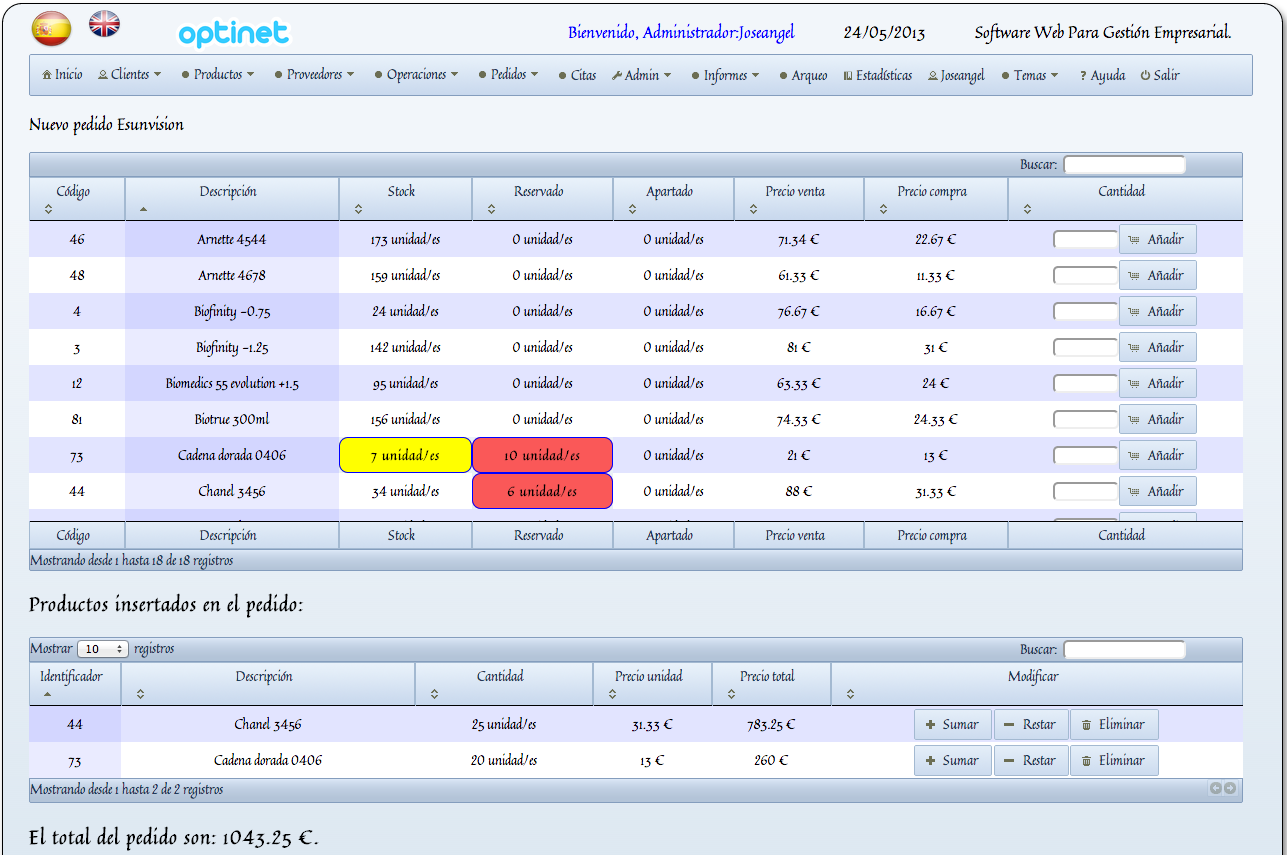
\includegraphics[scale=0.35]{capnuevopedido1.png}
  \caption{Pantalla nuevo pedido 1}
  \label{a}
\end{figure}

En esta pantalla el usuario introducirá los productos que quiere realizar al proveedor. Se mostrarán en un cuadro amarillo los productos con stocks menores que 10 y con un cuadro rojo los productos reservados, para que el usuario vea claramente las necesidades del sistema.

\newpage
\subsection {Pantalla listar pedidos}

\begin{figure}[!htb]
  \centering
    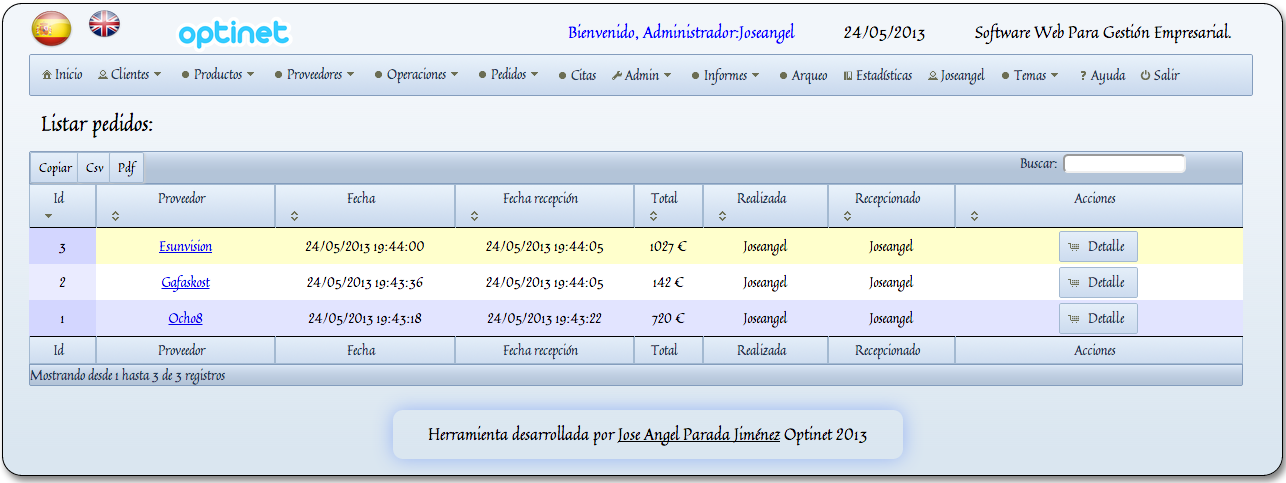
\includegraphics[scale=0.35]{caplistarpedidos.png}
  \caption{Pantalla listar pedidos}
  \label{a}
\end{figure}

En esta pantalla el usuario de la aplicación puede ver todos los pedidos realizados. Aquí es donde el usuario podrá recepcionar los pedidos realizados almacenándose el usuario que lo ha recepcionado, la fecha y actualizándose los stocks de los productos. También podrá ver los productos asociados a un pedido o mostrar el documento de pedido.

\subsection {Pantalla citas}

\begin{figure}[!htb]
  \centering
    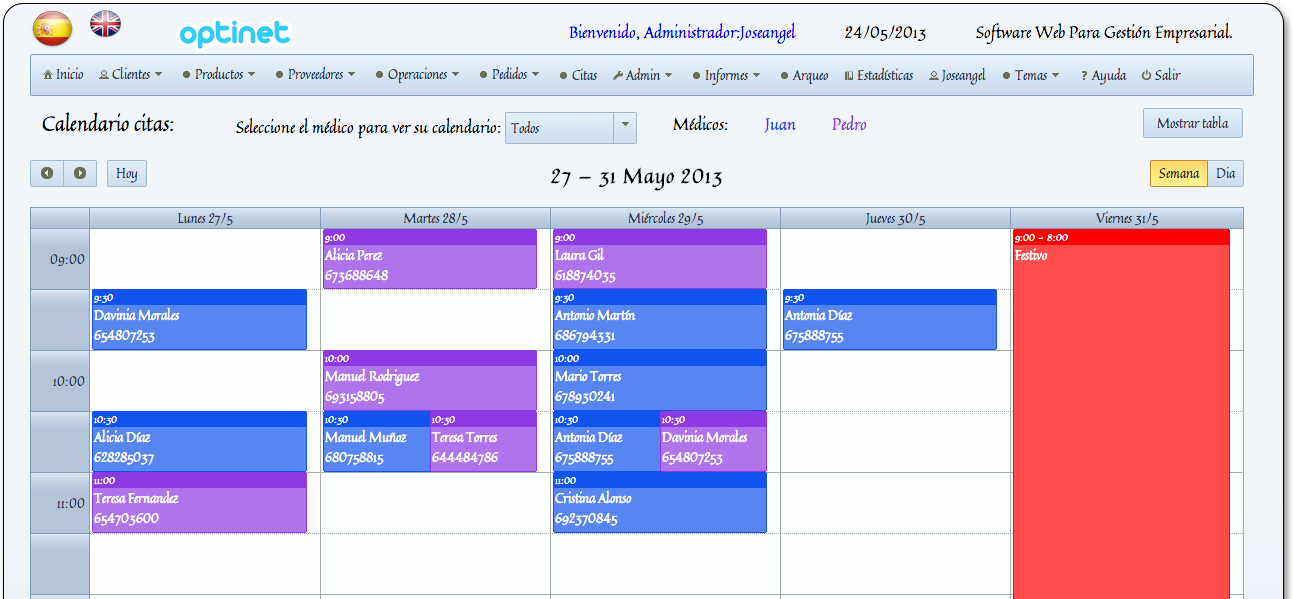
\includegraphics[scale=0.35]{capcitas.png}
  \caption{Pantalla citas}
  \label{a}
\end{figure}

En esta pantalla el usuario podrá gestionar las citas ya sea crear, eliminar o modificar una cita. El usuario tiene la posibilidad de mostrar en el calendario solo las citas de un determinado médico. Para eliminar una cita se pulsará en la cita y se mostrará un mensaje preguntando si se quiere verdaderamente eliminar la cita del sistema. Para realizar las búsquedas de citas más rápidamente o imprimir un documento de citas, se puede pulsar el botón mostrar tabla que aparece en la parte superior derecha de la pantalla. El sistema no dejará que se almacenen citas en días anteriores a la fecha actual. Los colores de las citas pertenecen al color asociado al médico que el administrador podrá cambiar en la pantalla modificación de empleado. Si se pulsase encima del día festivo, el sistema no permitiría crear una cita ya que no se puede crear citas en un día festivo.

\begin{figure}[!htb]
  \centering
    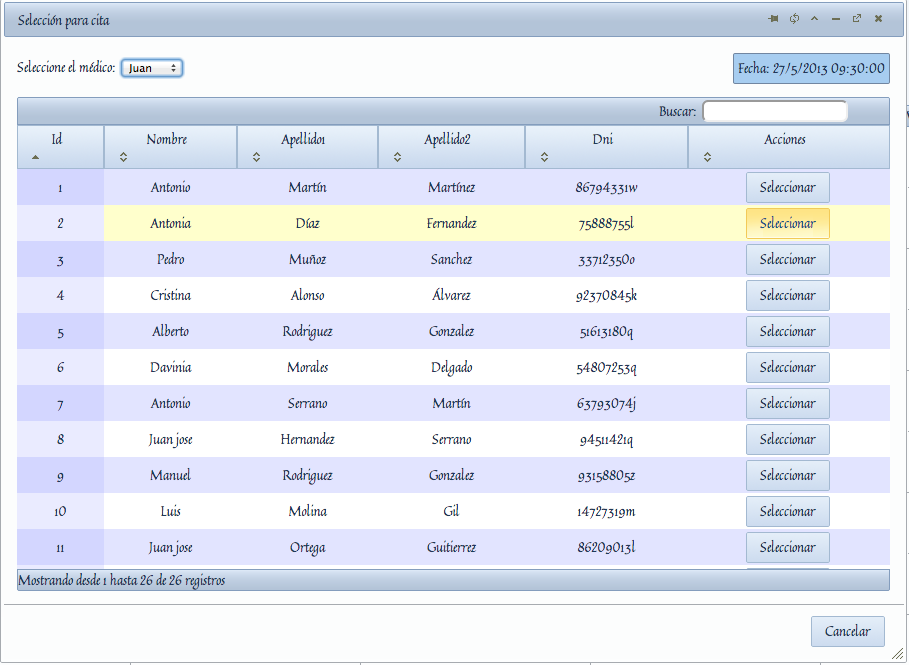
\includegraphics[scale=0.35]{capcitas1.png}
  \caption{Pantalla dialogo nueva cita}
  \label{a}
\end{figure}

En esta pantalla, que aparece al pulsar en una celda del calendario, se debe elegir a los participantes de la cita. El médico, que se podrá elegir en la parte superior izquierda, y que solo se mostrarán los médicos que estén disponibles(descartando los que tengan algún permiso en esa fecha o este desactivado). El cliente se podrá seleccionar en la tabla mediante el botón seleccionar. Si se escogiese un médico o cliente ocupado en esa fecha el sistema mostraría un error, no dejando almacenar la cita.

\newpage
\subsection{Pantalla registrar informe}
\begin{figure}[!htb]
  \centering
    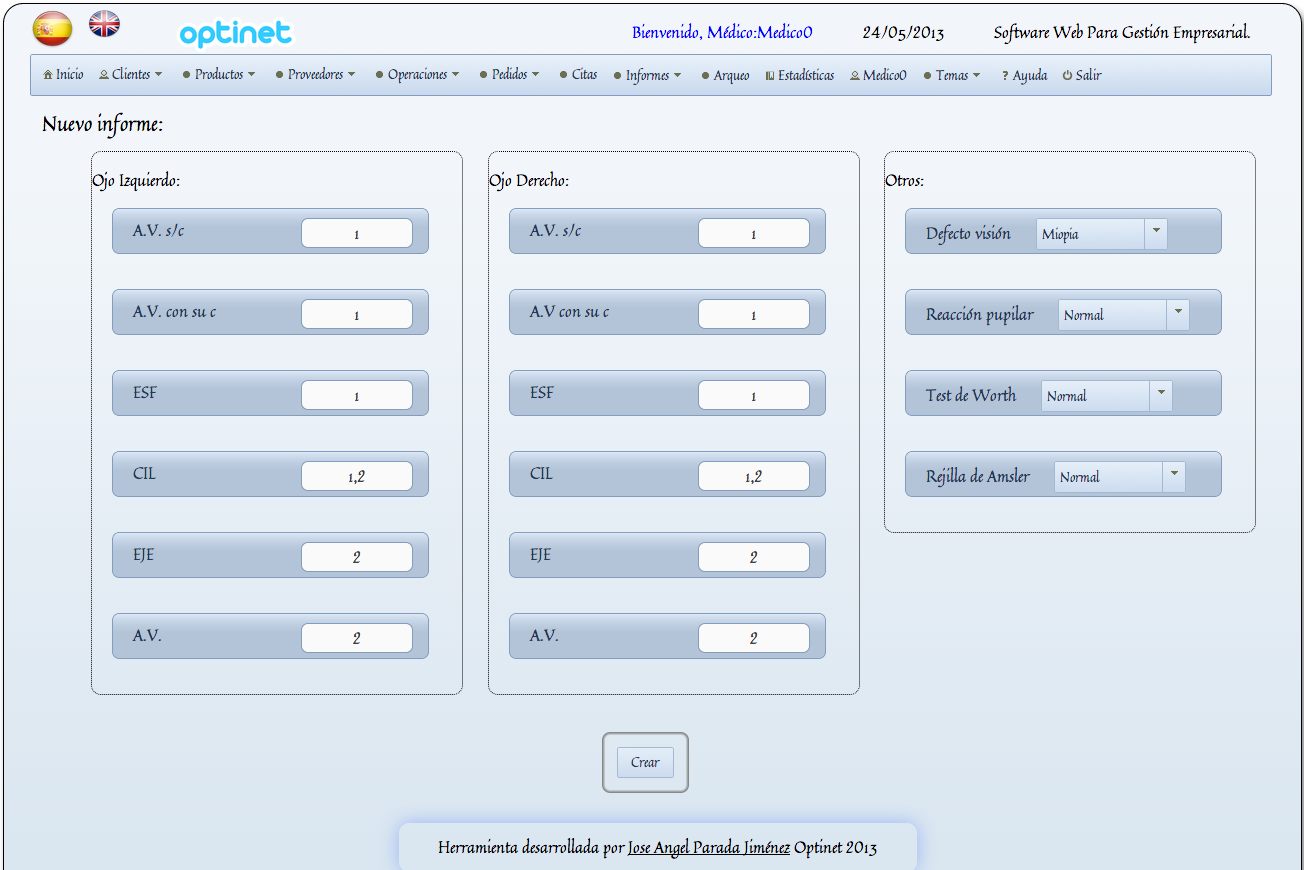
\includegraphics[scale=0.35]{capregistrarinforme.png}
  \caption{Pantalla nuevo informe}
  \label{a}
\end{figure}

Los informes solo lo pueden realizar los médicos y no son modificables. Los informes de los médicos se pueden realizar de dos maneras diferentes, con cita o sin cita.\\
 Si se eligiese la opción sin cita, se mostrará una tabla con los clientes almacenados en el sistema donde el usuario seleccionará al que quiere realizarle el informe. El sistema almacenará una cita en el momento de creación del informe.\\
Si se eligiese la opción con cita, se mostrará el calendario todas las citas asignadas al médico que esta conectado donde el médico seleccionará la cita a la que quiere realizarle el informe.\\

Las citas que ya tienen el informe realizado aparecerán en el calendario en color negro. Si se pulsase en cualquier cita que ya tiene informe se mostrará directamente el informe.

\newpage
\subsection {Pantalla registrar arqueo}

\begin{figure}[!htb]
  \centering
    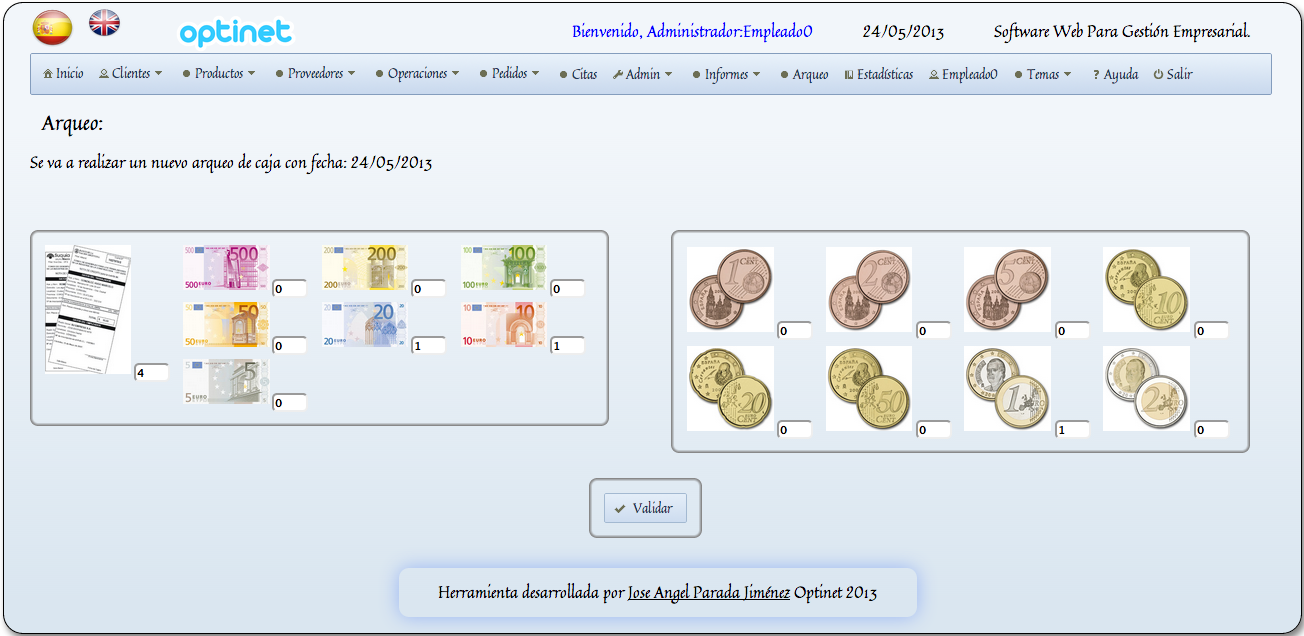
\includegraphics[scale=0.35]{capnuevoarqueo.png}
  \caption{Pantalla registrar arqueo}
  \label{a}
\end{figure}

En esta pantalla el usuario podrá realizar al final del día el recuento de la caja. El sistema no permitirá que se realice más de un arqueo diario mostrando un mensaje e invalidando el botón. El sistema mostrará un mensaje de error si detecta que no se han introducido de manera correcta los datos. Cuando el sistema hace la comprobación de la caja, si es correcto se almacena el arqueo en el sistema pero si por el contrario el arqueo difiere en más de 1 unidad mostrará un mensaje de arqueo NO confirmado ofreciendo la posibilidad al usuario de introducir de nuevo los datos o por el contrario guardar de todos modos.

\newpage
\subsection {Pantalla estadísticas usuario}

\begin{figure}[!htb]
  \centering
    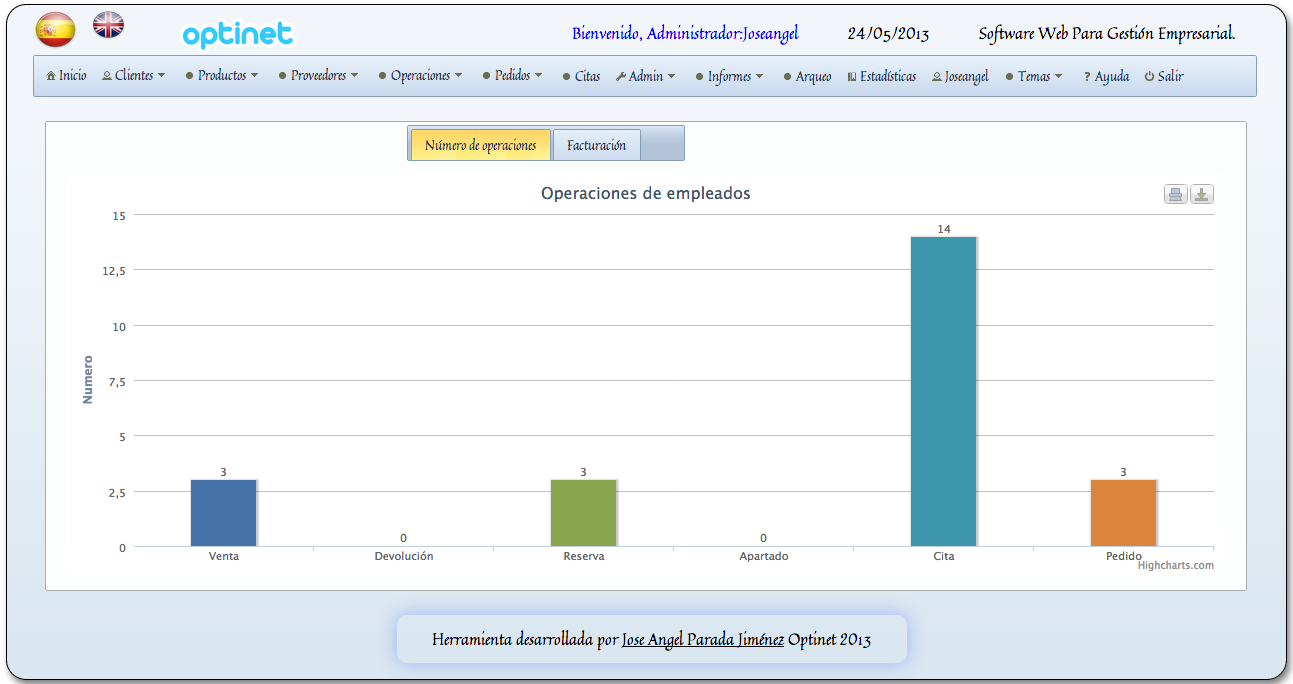
\includegraphics[scale=0.35]{capestadisticasemp.png}
  \caption{Pantalla estadísticas usuario}
  \label{a}
\end{figure}

En esta pantalla el usuario podrá navegar por el menú para ver sus propias estadísticas permitiendo, además, al usuario exportar las estadísticas a distintos formatos y la posibilidad de impresión. Si el usuario pulsará en cualquier barra del gráfico de mostraría el listado de las operaciones asociadas al gráfico.

\newpage
\subsection {Pantalla modificar usuario}

\begin{figure}[!htb]
  \centering
    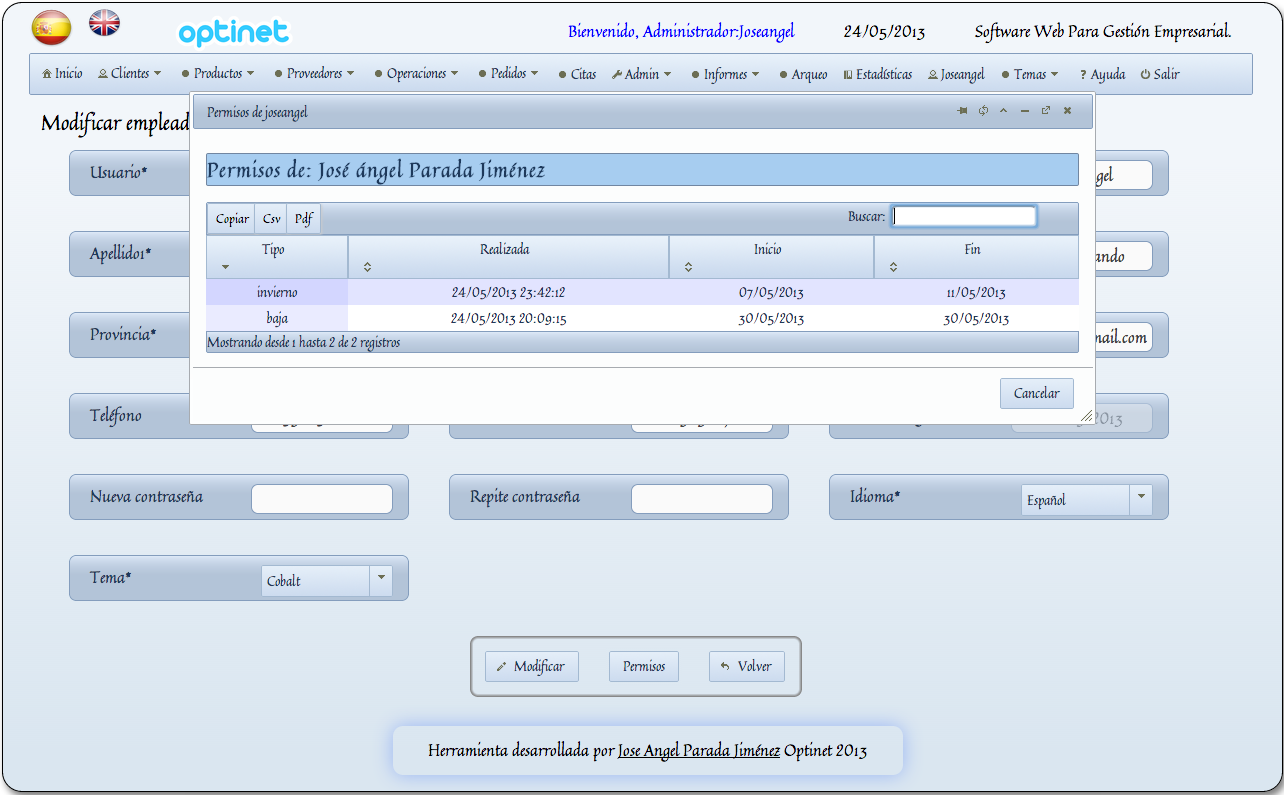
\includegraphics[scale=0.35]{capmodificarempleado.png}
  \caption{Pantalla modificar usuario}
  \label{a}
\end{figure}

En esta pantalla el usuario podrá modificar sus datos así como la contraseña. También ofrece la posibilidad de ver o imprimir los permisos que le ha asignado el administrador pulsando en el botón permisos. Si el usuario no tuviese ningún permiso, el botón aparecería desactivado.

\newpage
\subsection {Pantalla registrar empleado/médico}

\begin{figure}[!htb]
  \centering
    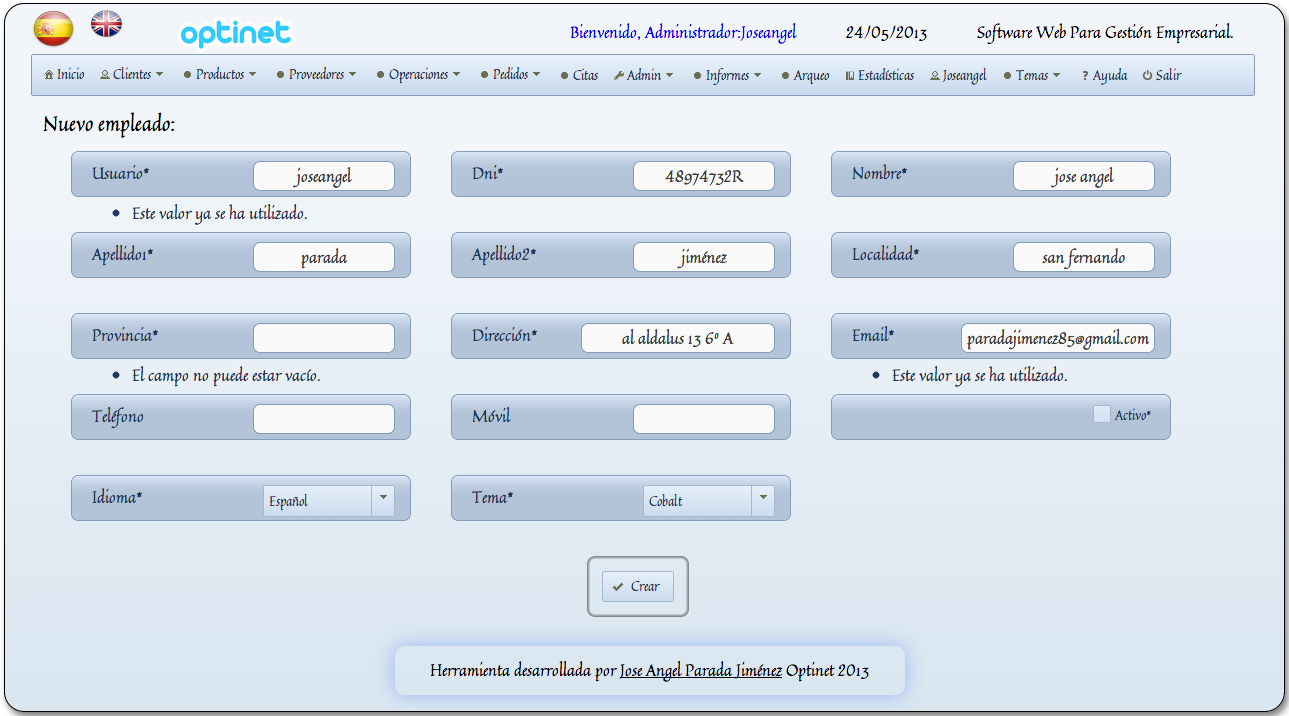
\includegraphics[scale=0.35]{capregistroemp.png}
  \caption{Pantalla registrar empleado/médico}
  \label{a}
\end{figure}

En esta pantalla el administrador podrá crear a un nuevo usuario de la aplicación. No se podrán crear dos usuarios con un mismo nombre de usuario o email y el sistema daría un error. Si el registro fuese de un médico aparecerán los campos adicionales titulación, número, color. El color es necesario ya que se pintarán las citas del médico con el color elegido en el calendario de citas.

\newpage
\subsection {Pantalla listar empleados}

\begin{figure}[!htb]
  \centering
    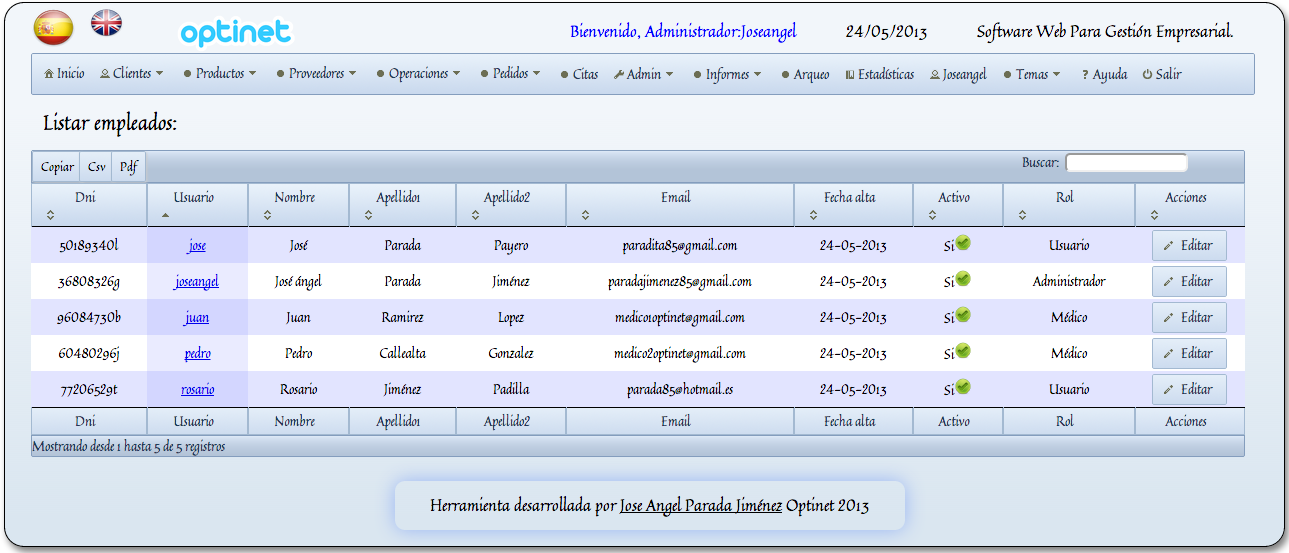
\includegraphics[scale=0.35]{caplistarempleados.png}
  \caption{Pantalla listar empleados}
  \label{a}
\end{figure}

En esta pantalla el administrador podrá consultar los usuarios de la aplicación. Se ofrece la posibilidad de editar a cualquier usuario de la aplicación excepto su contraseña, que solo la podrá saber el usuario. El administrador solo tiene la posibilidad de mandar de nuevo al email del usuario una contraseña nueva. El administrador es el único usuario de la aplicación que no se puede desactivar.

\subsection {Pantalla listar conexiones}

\begin{figure}[!htb]
  \centering
    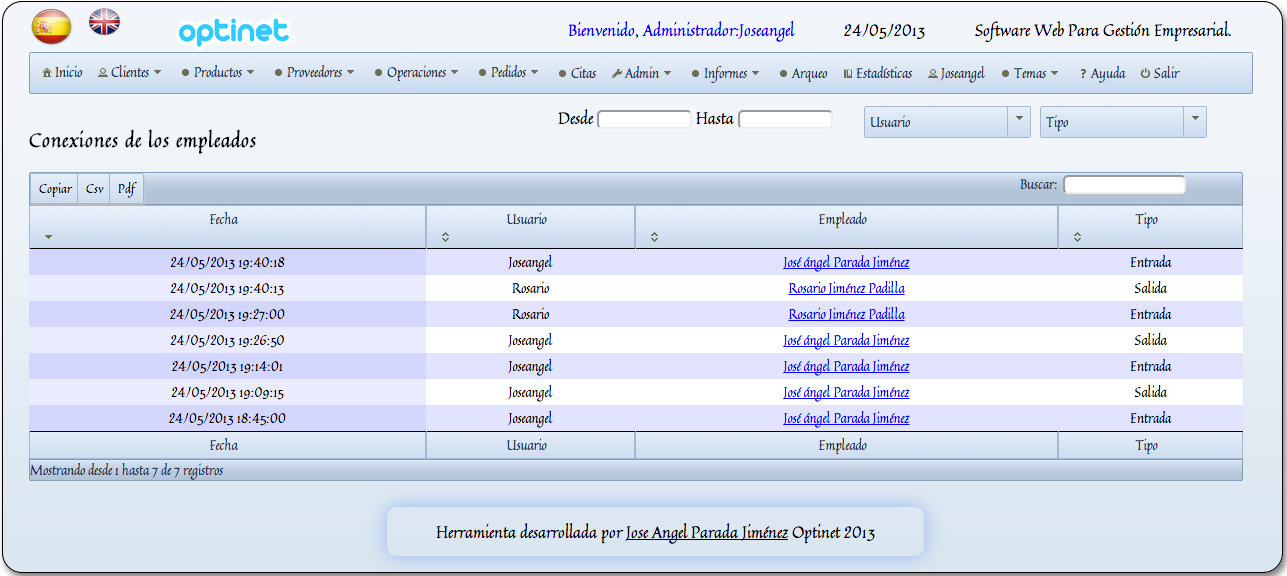
\includegraphics[scale=0.35]{capconexiones.png}
  \caption{Pantalla listar conexiones}
  \label{a}
\end{figure}

En esta pantalla el administrador podrá consultar las conexiones de los usuarios al sistema. De esta manera podrá tener información de la hora de entrada y salida al sistema de cada empleado.

\newpage
\subsection {Pantalla listar cambios}

\begin{figure}[!htb]
  \centering
    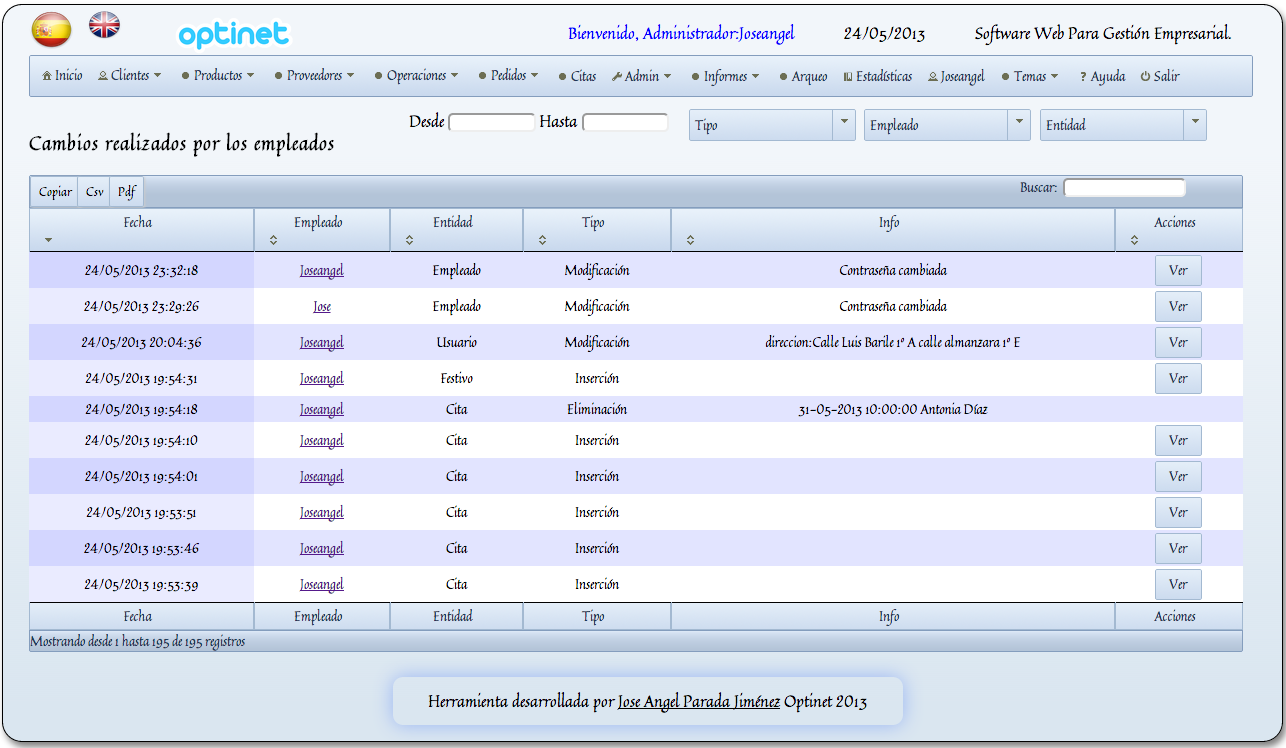
\includegraphics[scale=0.35]{capcambios.png}
  \caption{Pantalla listar cambios}
  \label{a}
\end{figure}

En esta pantalla el administrador podrá consultar los cambios efectuados al sistema. Si, por ejemplo, cambiásemos el nombre a un cliente quedaría almacenado en el sistema el nombre anterior y quien realizó el cambio, de esta manera el administrador sabrá en todo momento quien ha realizado cierto cambio en el sistema. Si el administrador o un usuario de la aplicación cambiase su contraseña, aparecería un mensaje de contraseña cambiada para que el administrador no pueda ver la contraseña del usuario.

\newpage
\subsection {Pantalla calendario arqueos}

\begin{figure}[!htb]
  \centering
    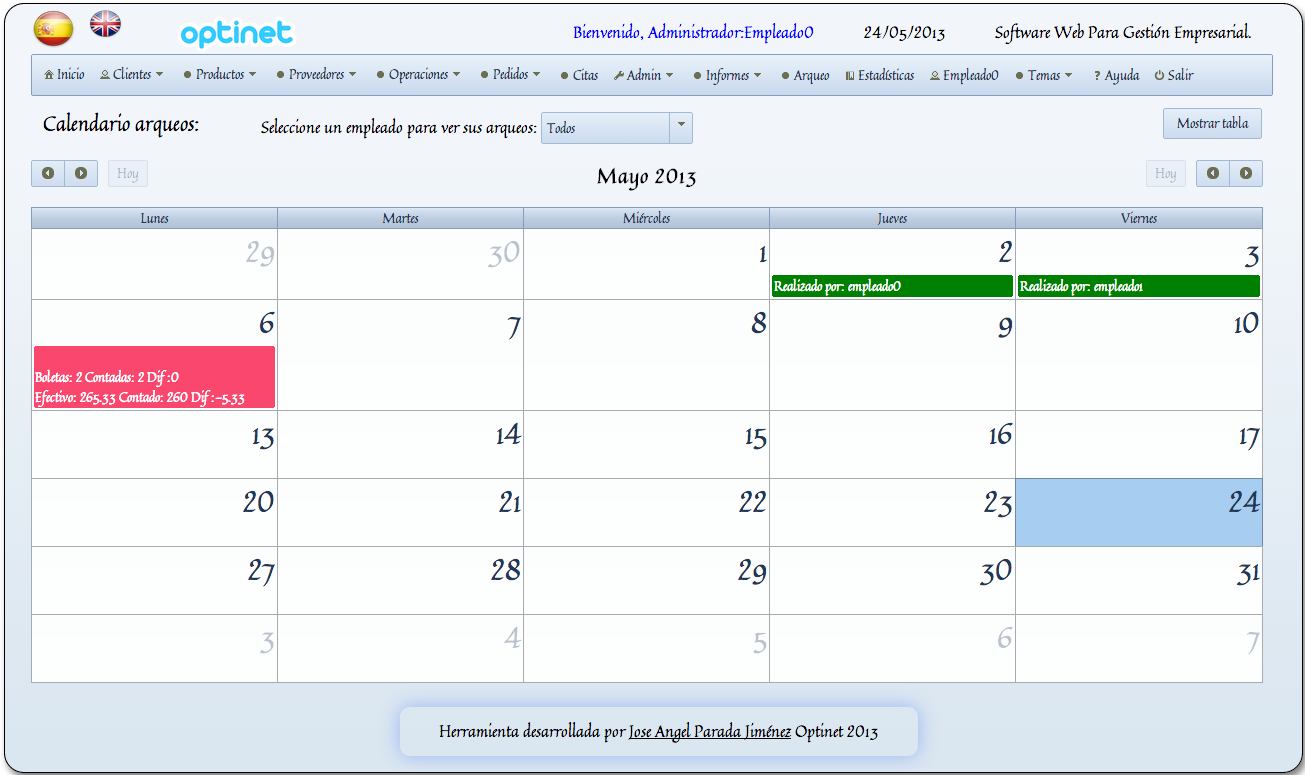
\includegraphics[scale=0.35]{capcalendarioarqueos.png}
  \caption{Pantalla calendario arqueos}
  \label{a}
\end{figure}

En esta pantalla el administrador podrá consultar los arqueos efectuados en el sistema. Los arqueos confirmados serán pintados en el calendario en color verde y los no confirmados de color rojo. Si dejásemos el puntero sobre cualquier arqueo, se mostrará la hora y quien realizó el arqueo. Para realizar búsquedas o simplemente imprimir una lista con los arqueos, podremos recurrir al botón de la parte superior derecha mostrar tabla donde aparecerán todos los arqueos.


\newpage
\subsection {Pantalla gestionar festivos}

\begin{figure}[!htb]
  \centering
    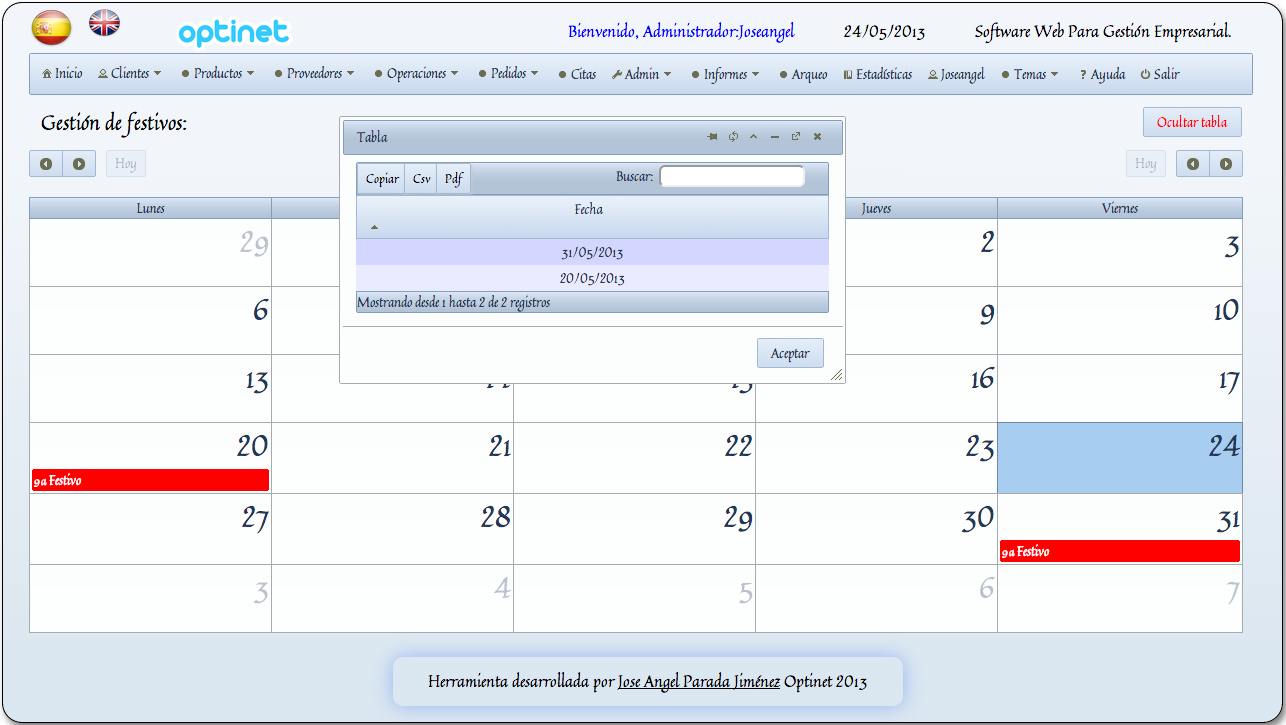
\includegraphics[scale=0.35]{capfestivos.png}
  \caption{Pantalla gestionar festivos}
  \label{a}
\end{figure}

En esta pantalla el administrador podrá gestionar los festivos. Para crear un nuevo festivo se pulsará en el día elegido. Para borrar un festivo se pulsará en el día festivo que se quiere borrar. No se podrá crear un día festivo en un día donde ya existan citas.Existe la posibilidad de mostrar una tabla con los festivos almacenados pulsando en el botón superior derecha mostrar tabla.

\newpage
\subsection {Pantalla gestionar permisos}

\begin{figure}[!htb]
  \centering
    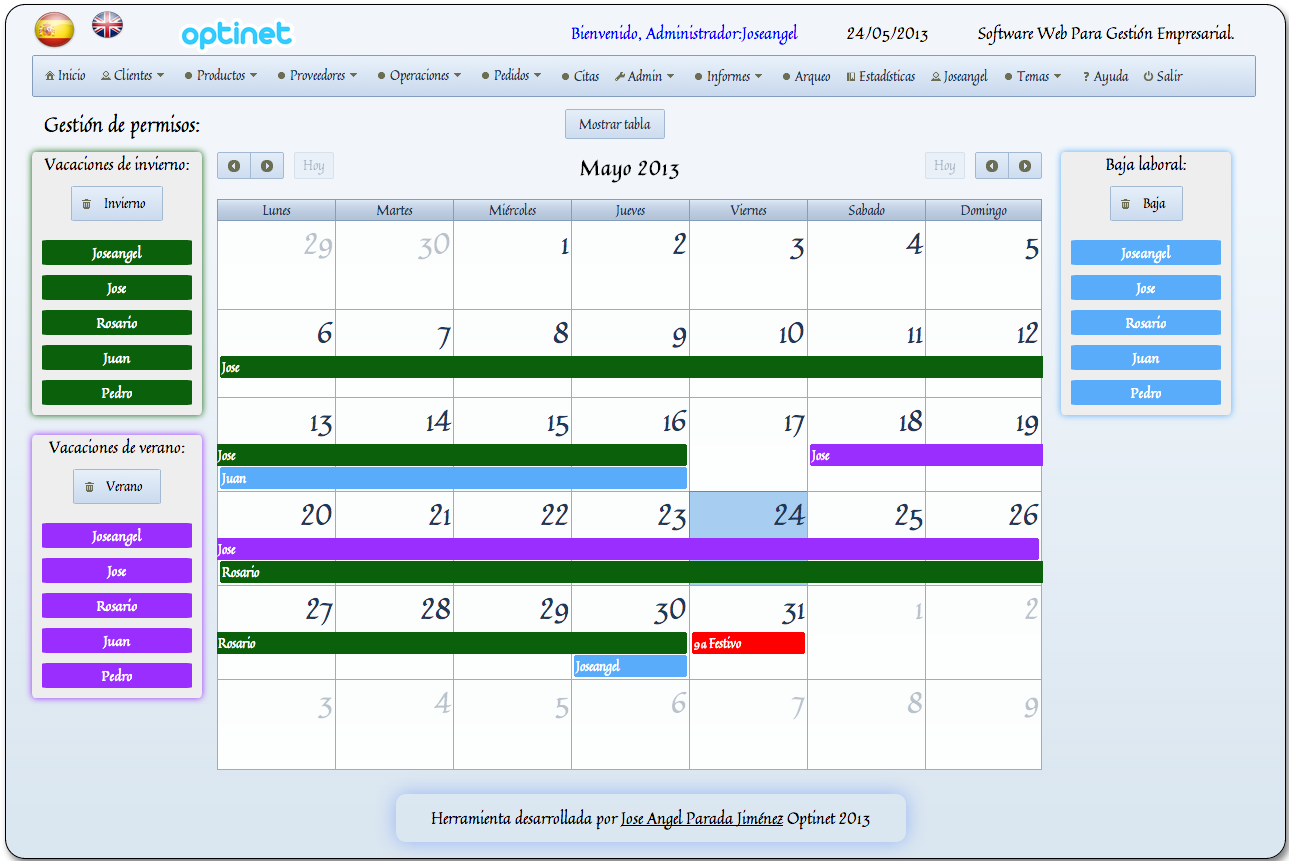
\includegraphics[scale=0.35]{cappermisos.png}
  \caption{Pantalla gestionar permisos}
  \label{a}
\end{figure}

En esta pantalla el administrador podrá gestionar los permisos asociados a los usuarios del sistema. Los permisos se asignarán arrastrándolos al calendario el día elegido. Los permisos se pueden alargar o acortar todo lo que uno desee. Se podrán eliminar los permisos pulsando sobre ellos, o si se quisiera borrar todos los permisos de un determinado tipo se pulsaría su botón correspondiente. Existe la posibilidad de mostrar los permisos en una tabla para así poder imprimirlos o, simplemente, buscar permisos más rápidamente. Existen algunas restricciones:
\begin{itemize}
\item No se puede crear unas mismas vacaciones en el mismo año. Ej: vacaciones invierno dos veces en el mismo año.
\item No puede tener un mismo empleado más de un permiso en la misma fecha. Ej. Una baja laboral y unas vacaciones de verano.
\end{itemize}

\newpage
\subsection {Pantalla estadísticas}

\begin{figure}[!htb]
  \centering
    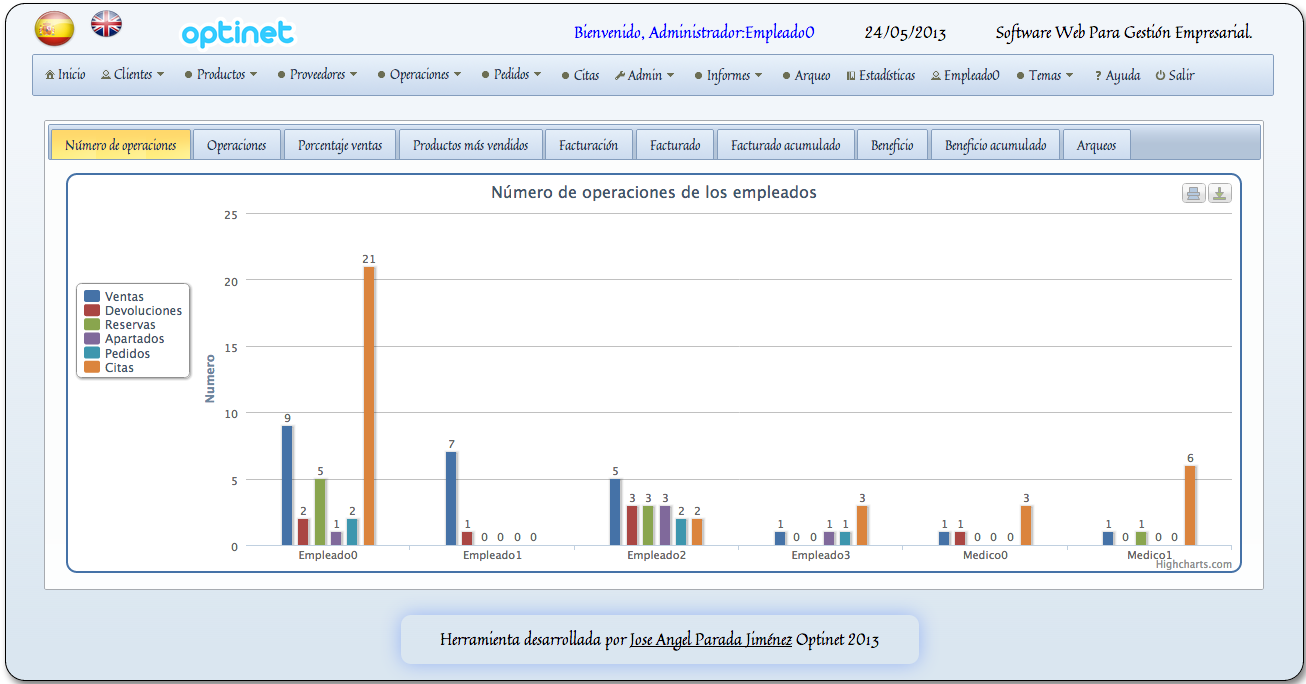
\includegraphics[scale=0.35]{capestadisticas.png}
  \caption{Pantalla estadísticas}
  \label{a}
\end{figure}

\begin{figure}[!htb]
  \centering
    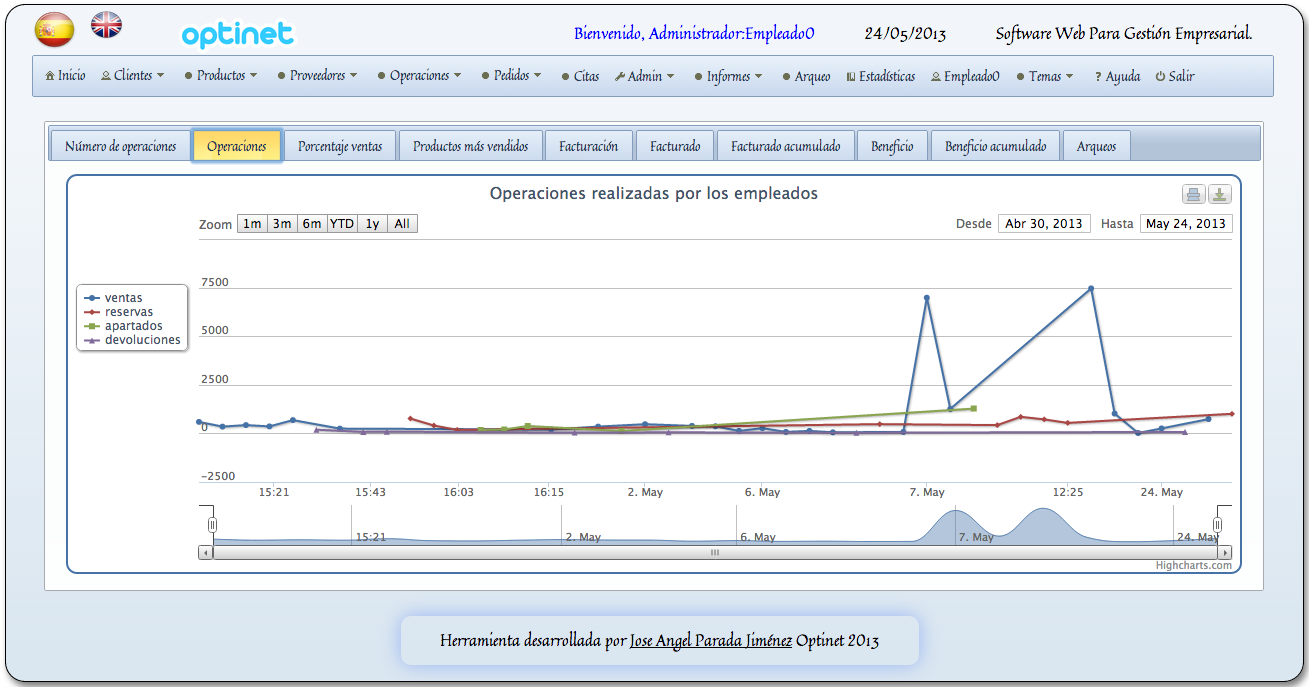
\includegraphics[scale=0.35]{capestadisticas1.png}
  \caption{Pantalla estadísticas 1}
  \label{a}
\end{figure}

\newpage
\begin{figure}[!htb]
  \centering
    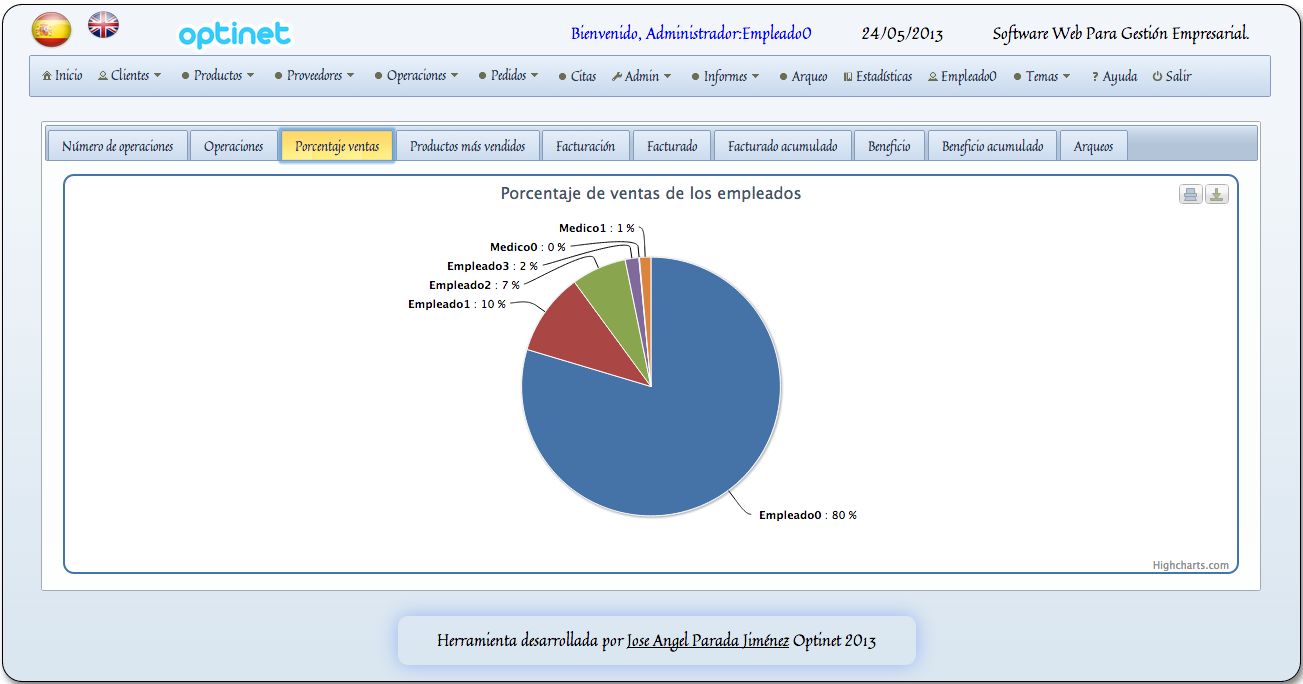
\includegraphics[scale=0.35]{capestadisticas2.png}
  \caption{Pantalla estadísticas 2}
  \label{a}
\end{figure}

\begin{figure}[!htb]
  \centering
    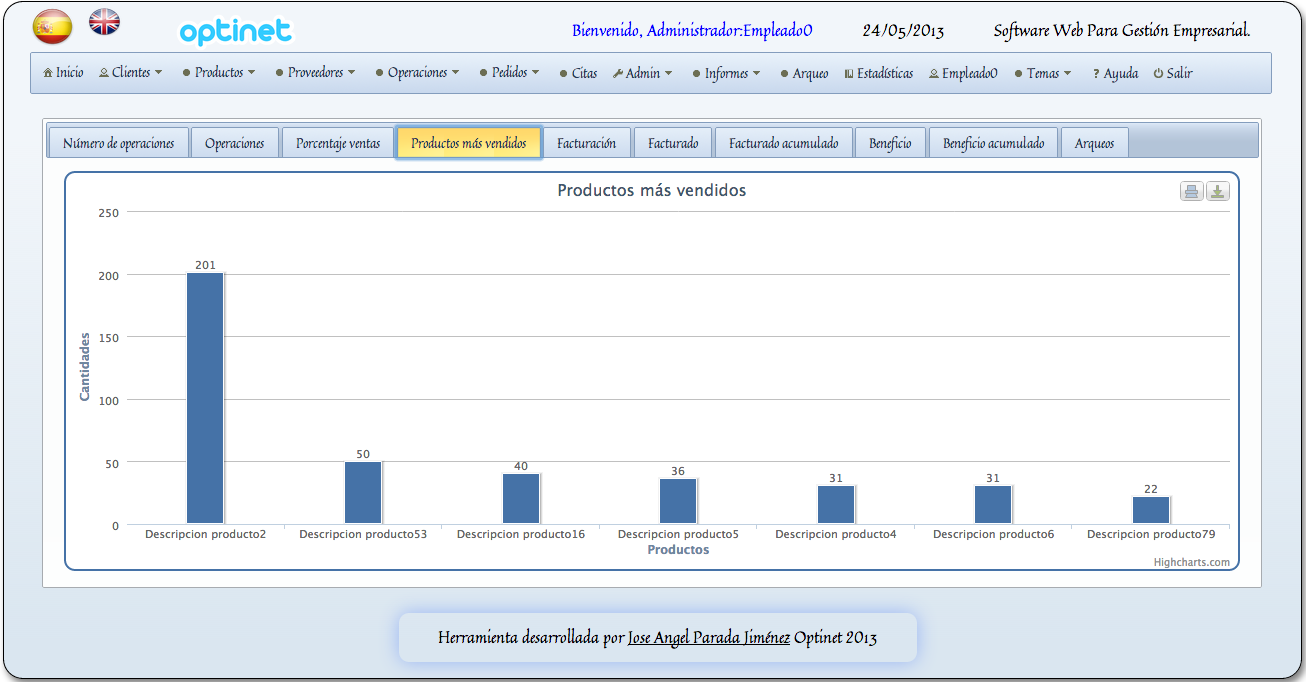
\includegraphics[scale=0.35]{capestadisticas3.png}
  \caption{Pantalla estadísticas 3}
  \label{a}
\end{figure}
En esta pantalla el administrador podrá consultar toda la información del sistema de manera gráfica. Todas las gráficas generadas ofrecen la posibilidad de imprimirlas o almacenarlas pulsando los iconos situados en la parte superior derecha. En el centro de la parte superior de la gráfica se muestra la descripción de cada gráfica.